\chapter{The Spanish electricity market}
In this section we briefly describe how the wholesale electricity market works in Spain.
In 1998, the current regulation came into operation, replacing the previous system in which Red Eléctrica de España (REE) and the Ministry of Industry and Energy entirely planned their transactions.

It allowed the private sector to freely plan the construction of generation plants and the possibility of bidding energy prices, and created the figure of energy supplier (being the consumer able to choose one).
Distribution of energy remained regulated by the government, who assigns this task to a unique company per region. \cite{mercado-electrico-mincotur}

The wholesale electricity market differs from the retail market. In the former generators sell energy to suppliers, while in the latter suppliers sell energy to consumers. Different agents participate in both, and they are regulated by different rules, being more flexible in the retail market.

\section{Main agents}
Different agents conform this complex system. Each one is in charge of a specific task:\cite{mercado-electrico-endesa, organismos-reguladores-holaluz}

\begin{itemize}
    \item \textbf{Generators} produce energy and should build, operate and maintain the power plants.
    \item \textbf{Transporters} take the energy from the power plants to the distribution network, building and maintaining the transport network. This network operates in high voltage, making transmission through long distances more efficient.
    \item \textbf{Distributors} extract the energy from the transport network and supply it to the final consumers. They are in charge of building and maintaining the distribution network.
    \item \textbf{Suppliers} buy the energy to generators and sell it to final consumers.
    \item \textbf{Regulators} are in charge of legislating (government administration) and ensuring effective competition (Comisión Nacional de los Mercados y la Competencia, CNMC) in the energy market.
    \item There exist two \textbf{operators}, the market operator and the system operator. The former (Operador de Mercado Ibérico de Energía, OMIE) manages the day-ahead and intraday electricity markets. The latter (Red Eléctrica de España, REE) ensures the system stability, checking that generation and consumption are balanced every time as energy can't be stored in large scale, preventing lack of supply or overload on the power grid. Both operators should work closely, so they can face adequately to problems in the system.
\end{itemize}

\section{The electricity price}
The main goal of this Thesis is to study electricity market prices.
These are the prices which supplying companies pay for the energy, and not the final price each consumer pays when using, for example, the Precio Voluntario Pequeño Consumidor (PVPC) tariff, which also includes regulated costs and taxes. \cite{mercado-electrico-xataka}

The prices for next day are fixed in the electricity market or pool, which happens every day at 12 pm.
On it, suppliers make their purchase bids, which are ordered from lower to higher in the supply curve (green curve in Figure \ref{fig:supply-demand-curves})
On the other hand, generators make their sell bids which are ordered from higher to lower in the demand curve (blue curve in Figure \ref{fig:supply-demand-curves}).

\begin{figure}[H]
\centering
    \caption{Energy supply and demand curves in the wholesale market. \cite{curva-oferta-demanda}}
    \label{fig:supply-demand-curves}
    \fbox{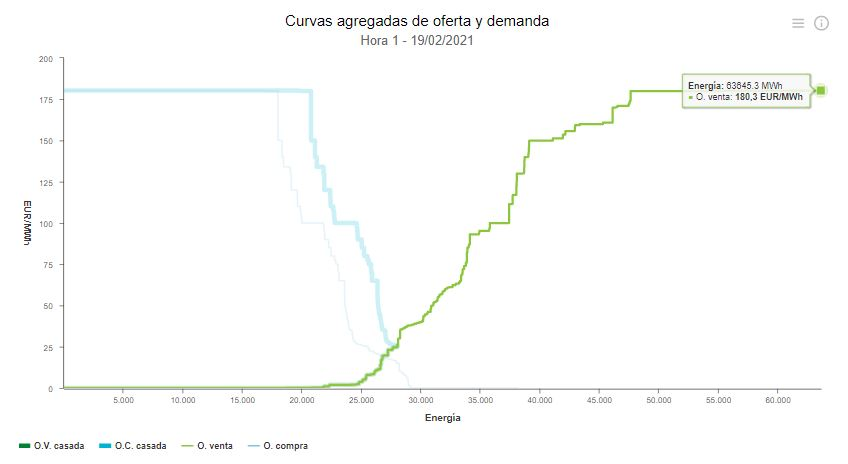
\includegraphics[scale=0.6]{images/supply-demand-curves.jpeg}}
\end{figure}

The point where the two curves intersect defines the price at which energy will be sold. On the left of this intersection appear the transactions that will take place, while those on the right will not be materialized, as the generators ask for more money than what suppliers are willing to pay.
All the sold electricity will be available at that intersection price, the generators will receive that price even if they bid for less.

These characteristics are what define a marginal pricing market.
This process will be repeated for each hour of the following day, having a total of 24 different prices.

This variable will be obtained both from ESIOS (short term) and OMIE (long term): both data sources contain the same information, as prices are built in a regulated basis as explained in the previous paragraphs. The data acquired goes from 01-1998 to 03-2023, in an hourly fashion.

Let's visually analyze the data in Figure \ref{fig:spot-price-series}. On an hourly scale, the author appreciates some cyclicity happening every 12 hours, something that can be confirmed in the ACF plot.
Concretely, peaks in price appear at the early morning and in the evening.
During the night and late morning the price goes down: this could be due to our daily routines, as we consume less energy while we sleep or while we are working.
Nevertheless, we will know more about this in the future sections, when we study the predictor's importance.
On a monthly scale the author doesn't find cyclicity. But it is interesting to mention the peak in prices between 2021 and 2023 due to the war in Ukraine, as Europe is very dependent of fossil fuels imported from Russia \cite{lopez2022geopolitica}.

\begin{figure}[H]
\centering
    \begin{subfigure}{.45\textwidth}
        \centering
        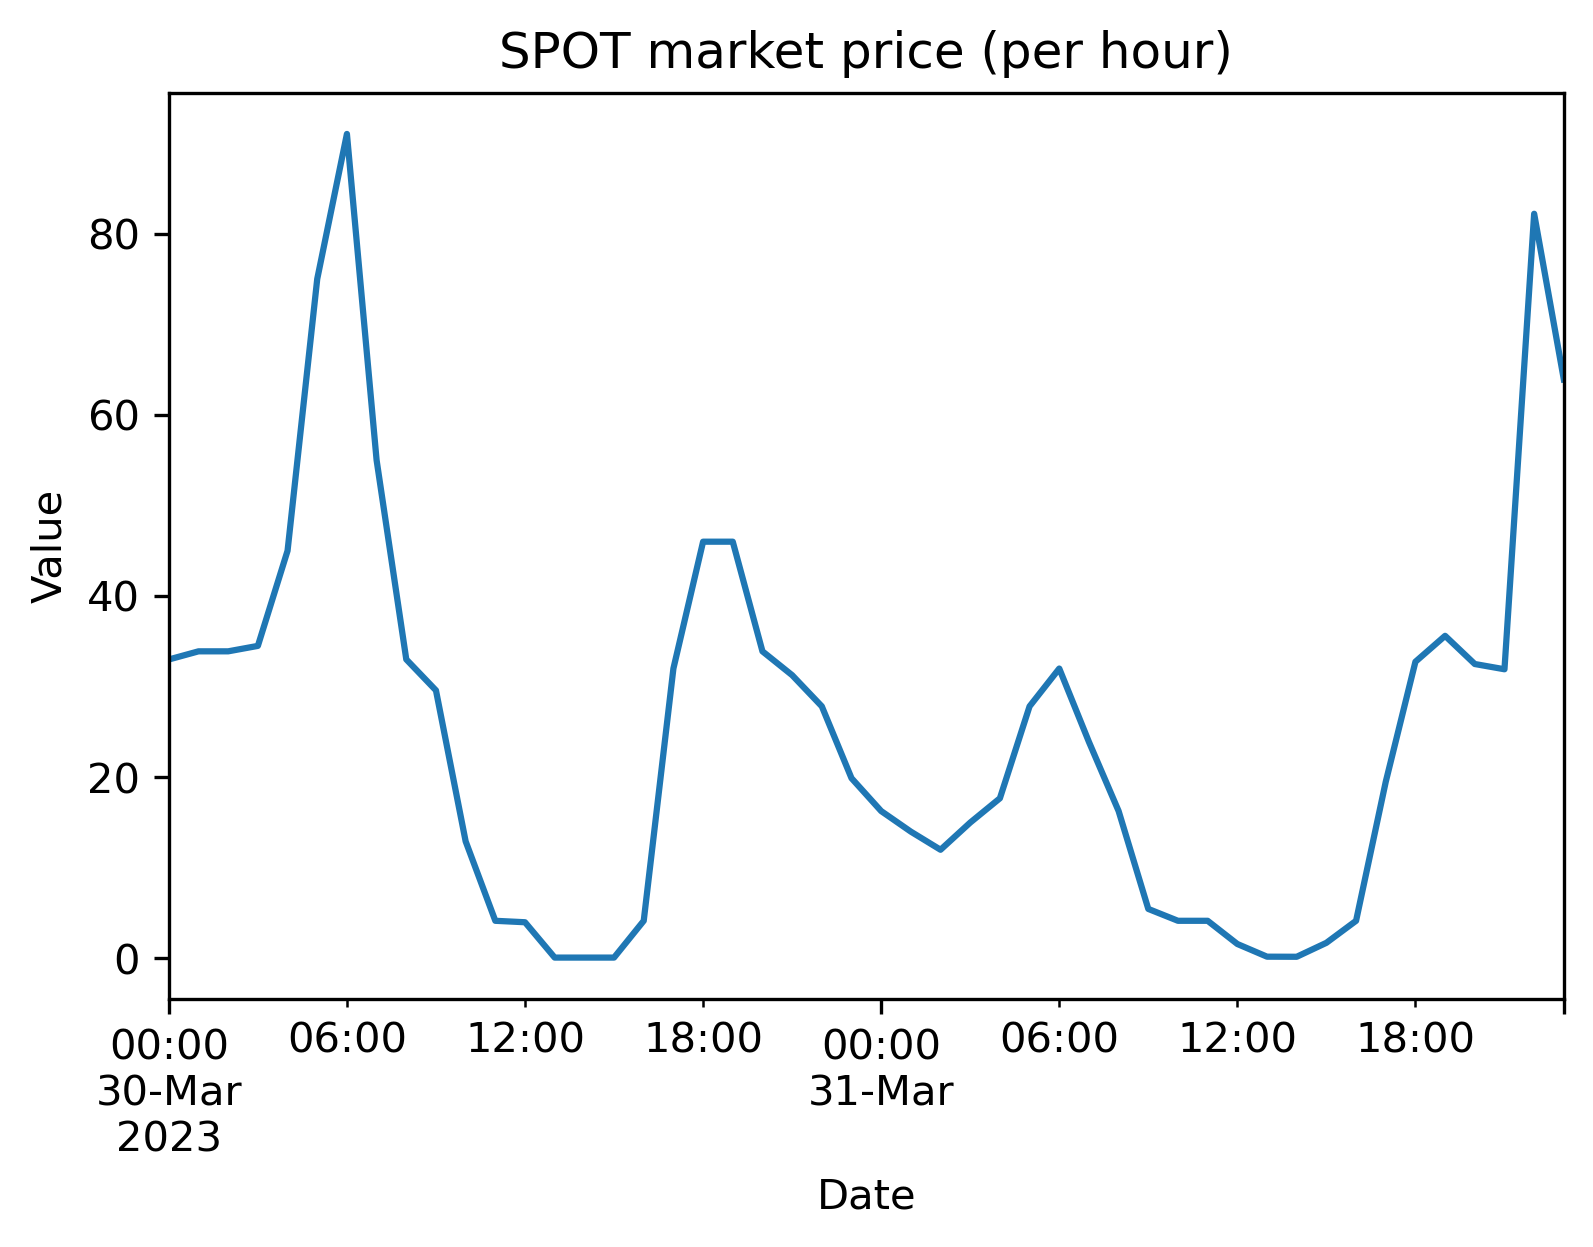
\includegraphics[width=1\linewidth]{images/variable_analysis/esios_spot_h_48}
        \caption{Per hour, 48 hours window.}
    \end{subfigure}
    \begin{subfigure}{.45\textwidth}
        \centering
        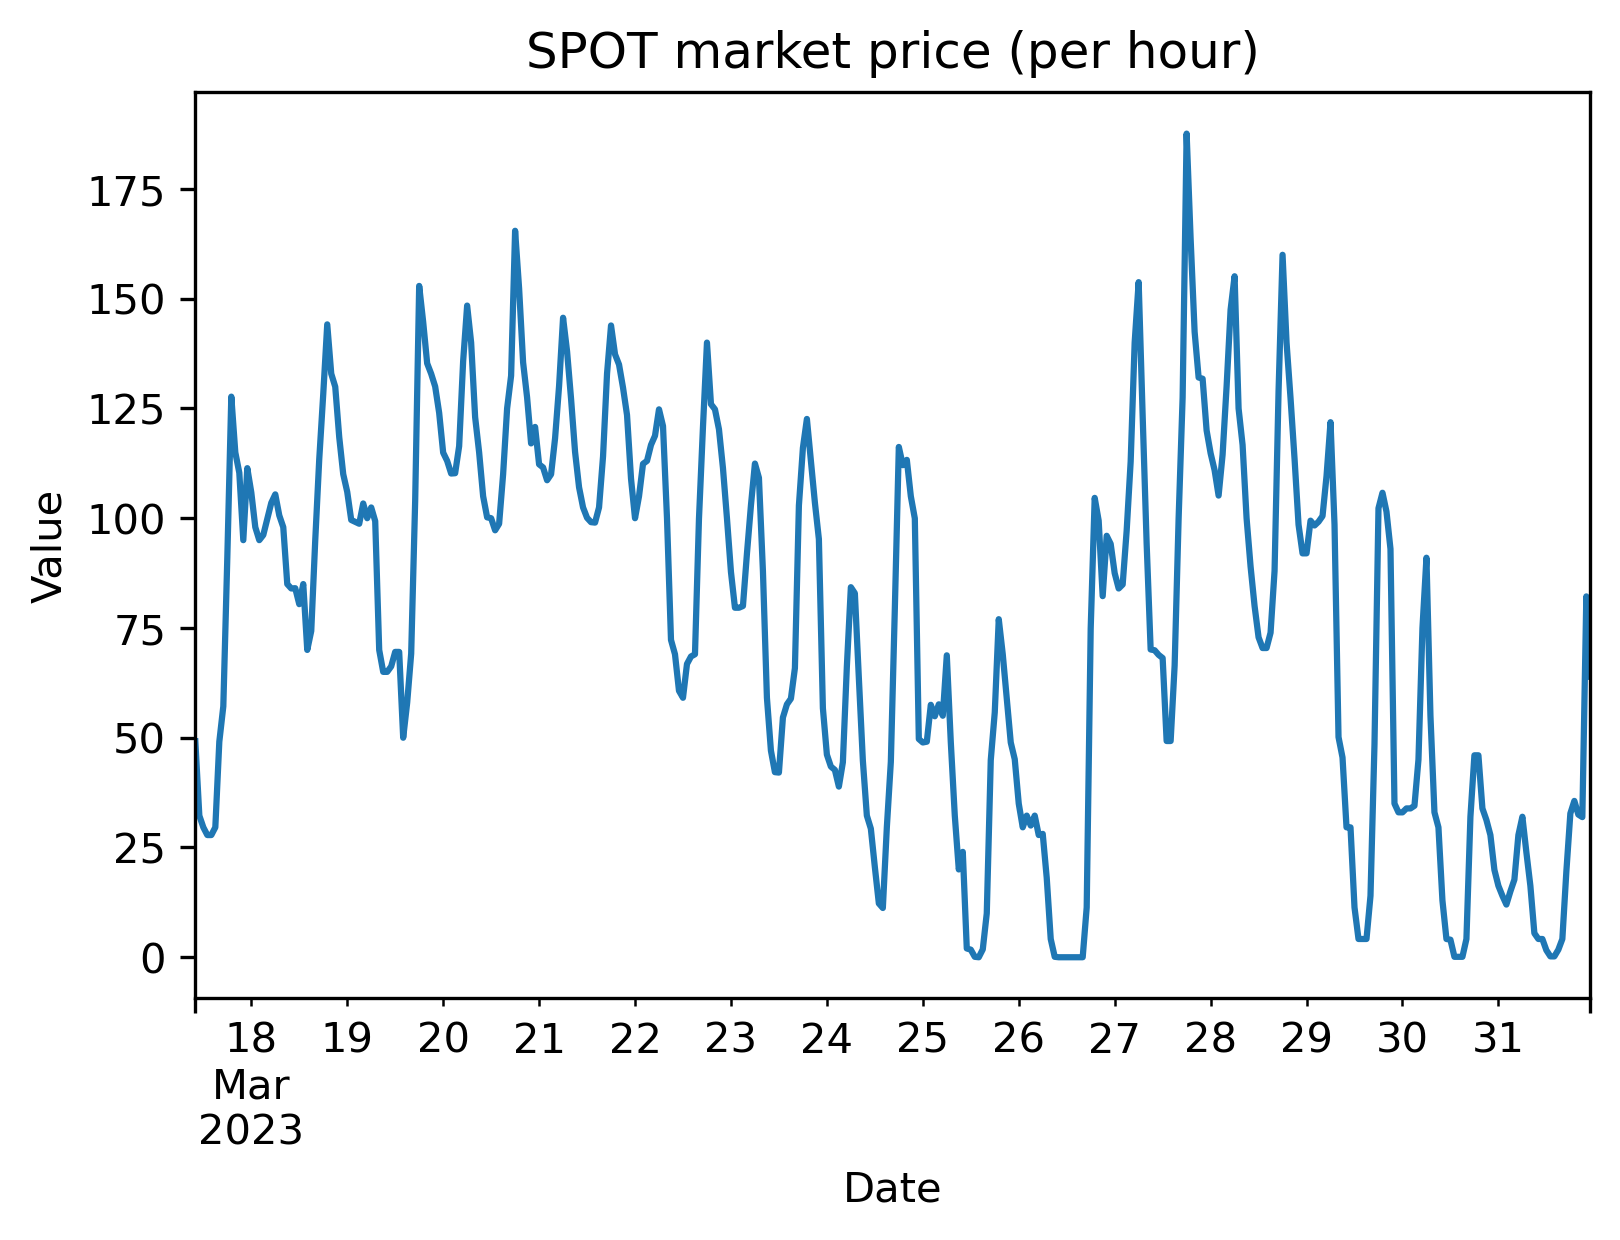
\includegraphics[width=1\linewidth]{images/variable_analysis/esios_spot_h_350}
        \caption{Per hour, 350 hours window.}
    \end{subfigure}
\end{figure}

\begin{figure}[H]\ContinuedFloat
    \begin{subfigure}{.45\textwidth}
        \centering
        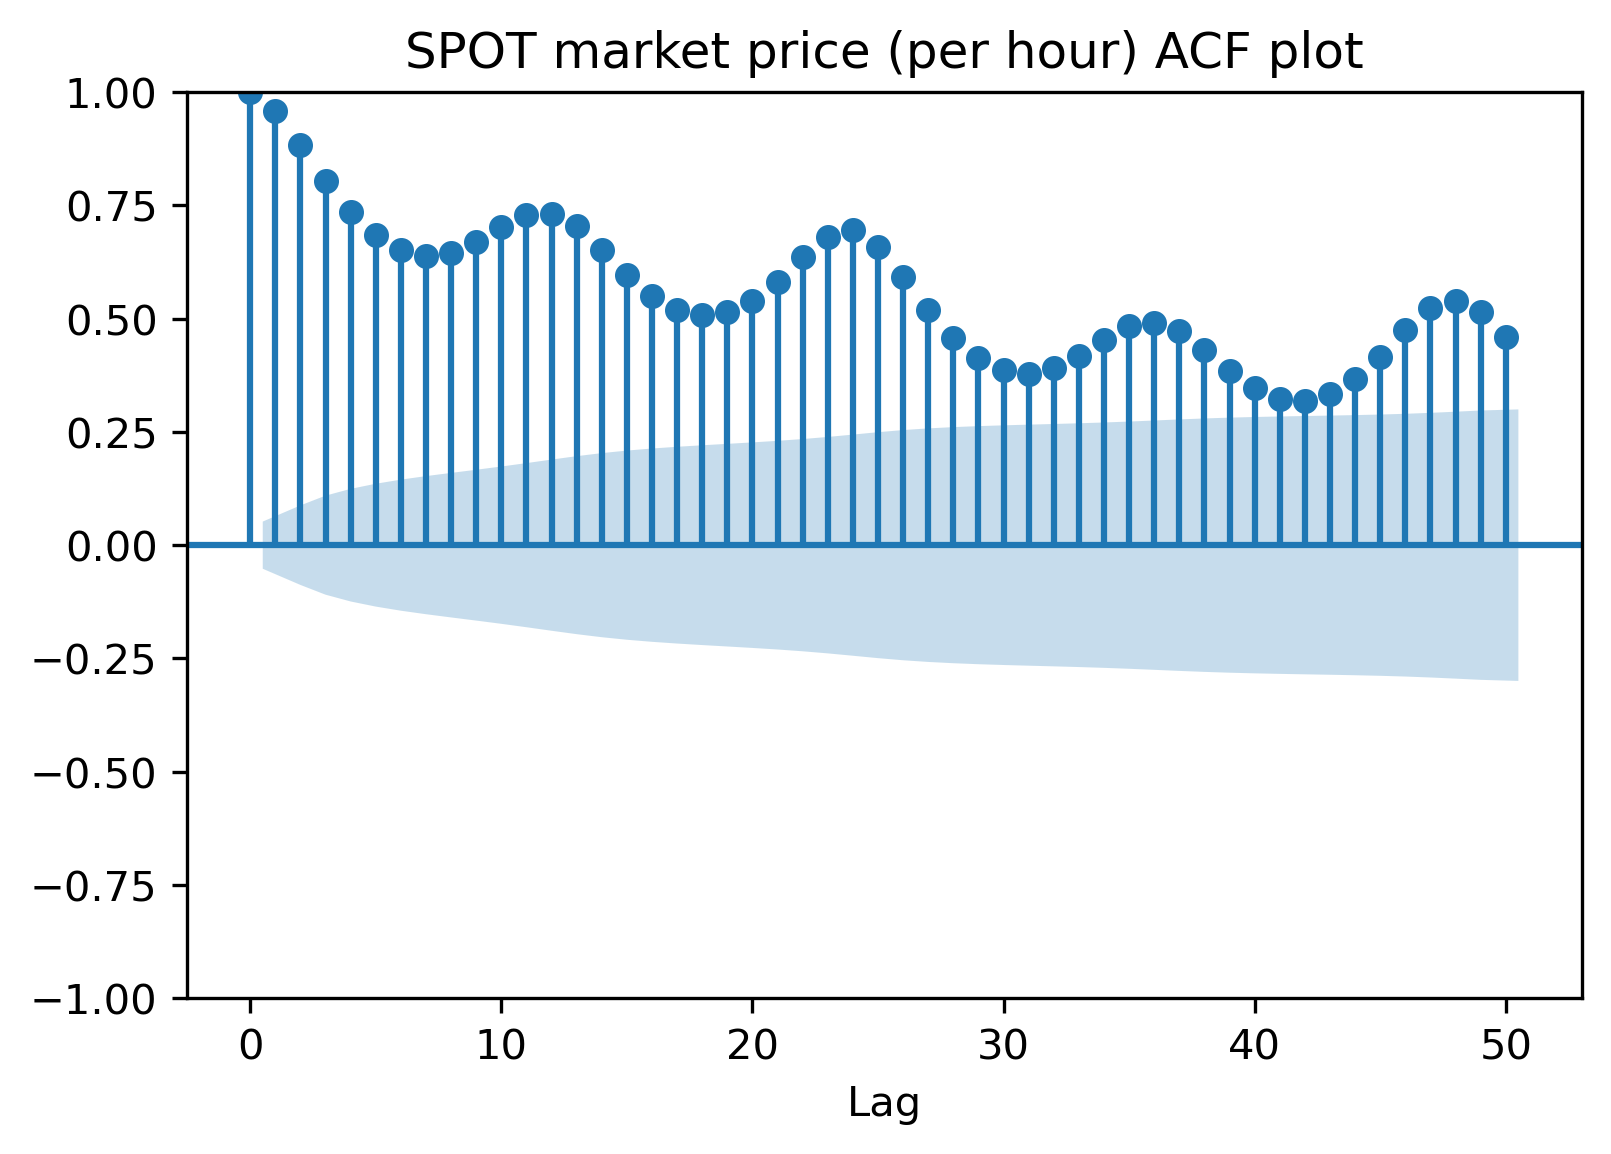
\includegraphics[width=1\linewidth]{images/variable_analysis/esios_spot_h_acf}
        \caption{ACF plot with 50 lags.}
    \end{subfigure}
    \begin{subfigure}{.45\textwidth}
        \centering
        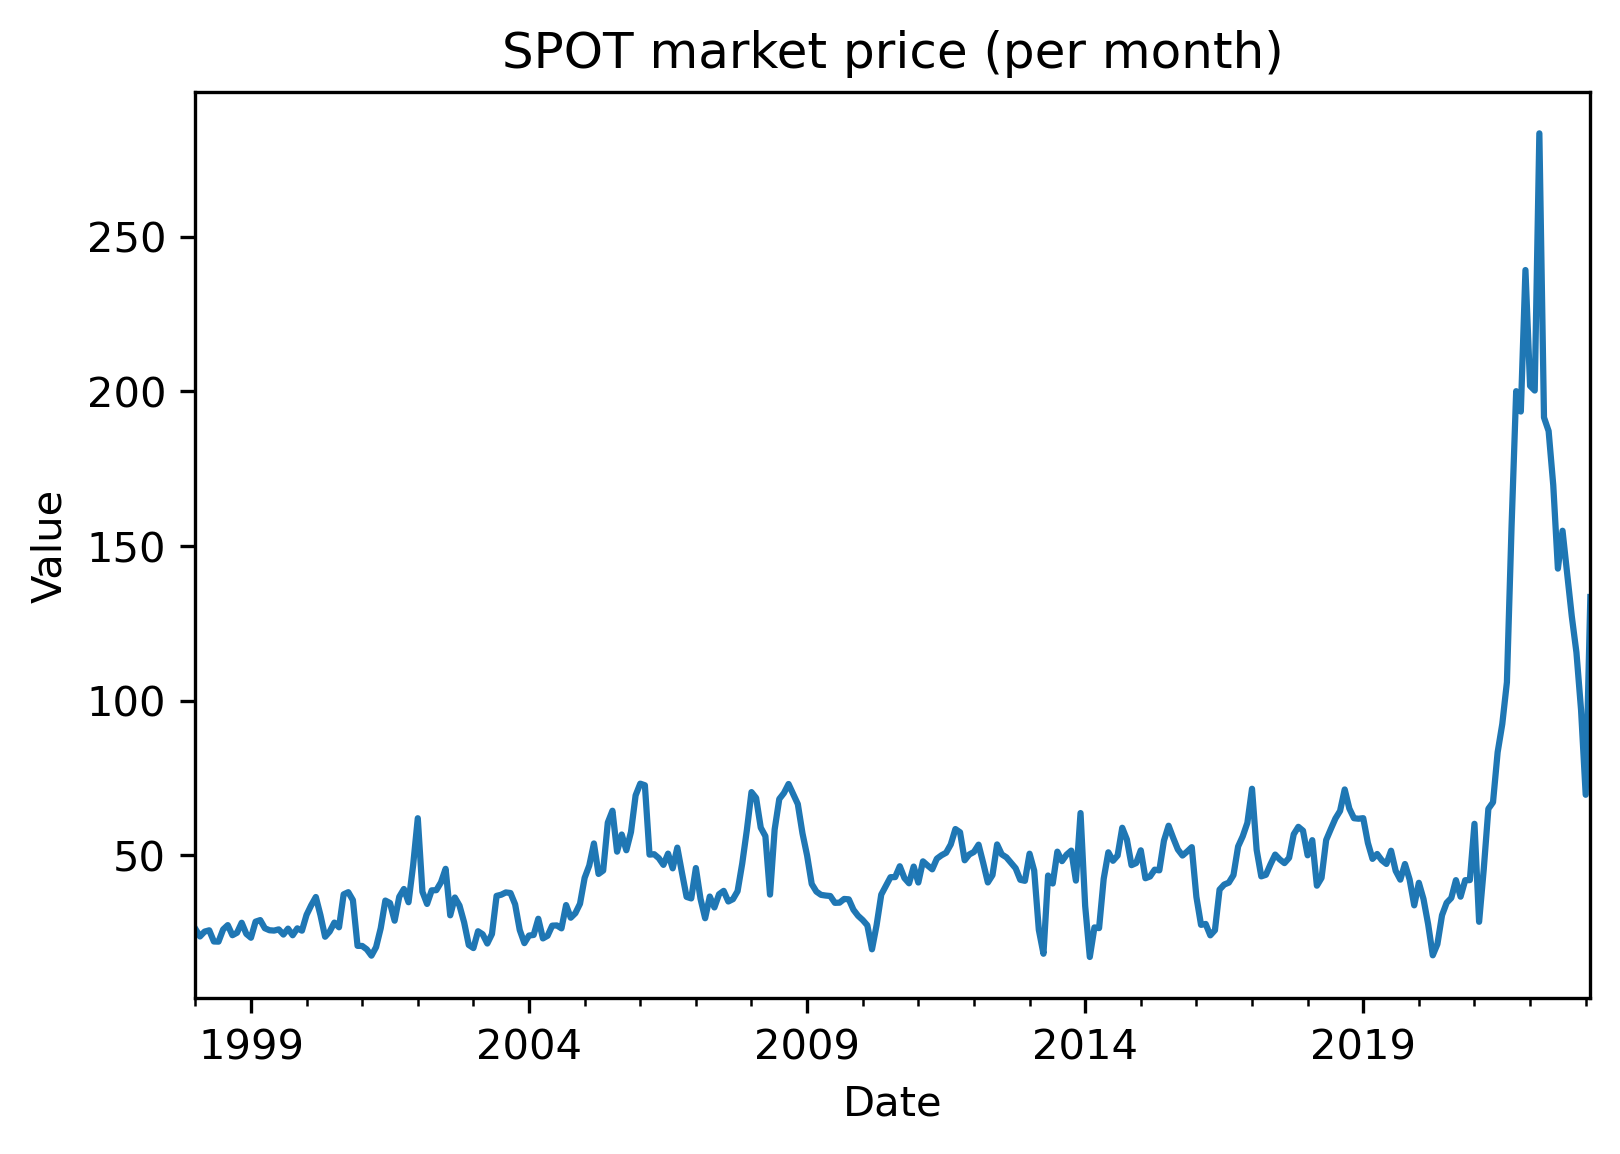
\includegraphics[width=1\linewidth]{images/variable_analysis/esios_spot_m_omie_all}
        \caption{Aggregated by month.}
    \end{subfigure}

    \caption{Electricity market SPOT price curves analysis.}
    \label{fig:spot-price-series}
\end{figure}

\section{Variables affecting the electricity price}
As the price is built in the free market, defining a priori the variables that influence it is difficult.
Many factors can affect its value, even companies strategic decisions that can't be predicted, but there are some variables that could fit in the equation that will be described in the following subsections. \cite{mercado-electrico-periodico-energia, mercado-electrico-cambio-energetico}

\subsection{Demand}
The energy consumption can affect the price, specially in a marginal pricing market.
As generation bids are ordered in the supply curve from cheaper to expensive, if the demand is high the intersection point will probably move to the right leading to a higher price.
The measured demand curves have been downloaded from ESIOS, obtaining data from 01-2014 to 03-2023. The granularity they originally have is of one reading every 10 minutes, but the author has aggregated this into hourly measurements.

If we study the plots in Figure \ref{fig:demand-series} we find how there is cyclicity at a daily level, there are repeating patterns each 24 hours, which makes sense due to people daily routines. There is also weekly cyclicity, existing higher consumption during the work days than during the weekends: this could be related with industry energy demand. It is also happening at yearly and half-yearly levels.

\begin{figure}[H]
\centering
    \begin{subfigure}{.435\textwidth}
        \centering
        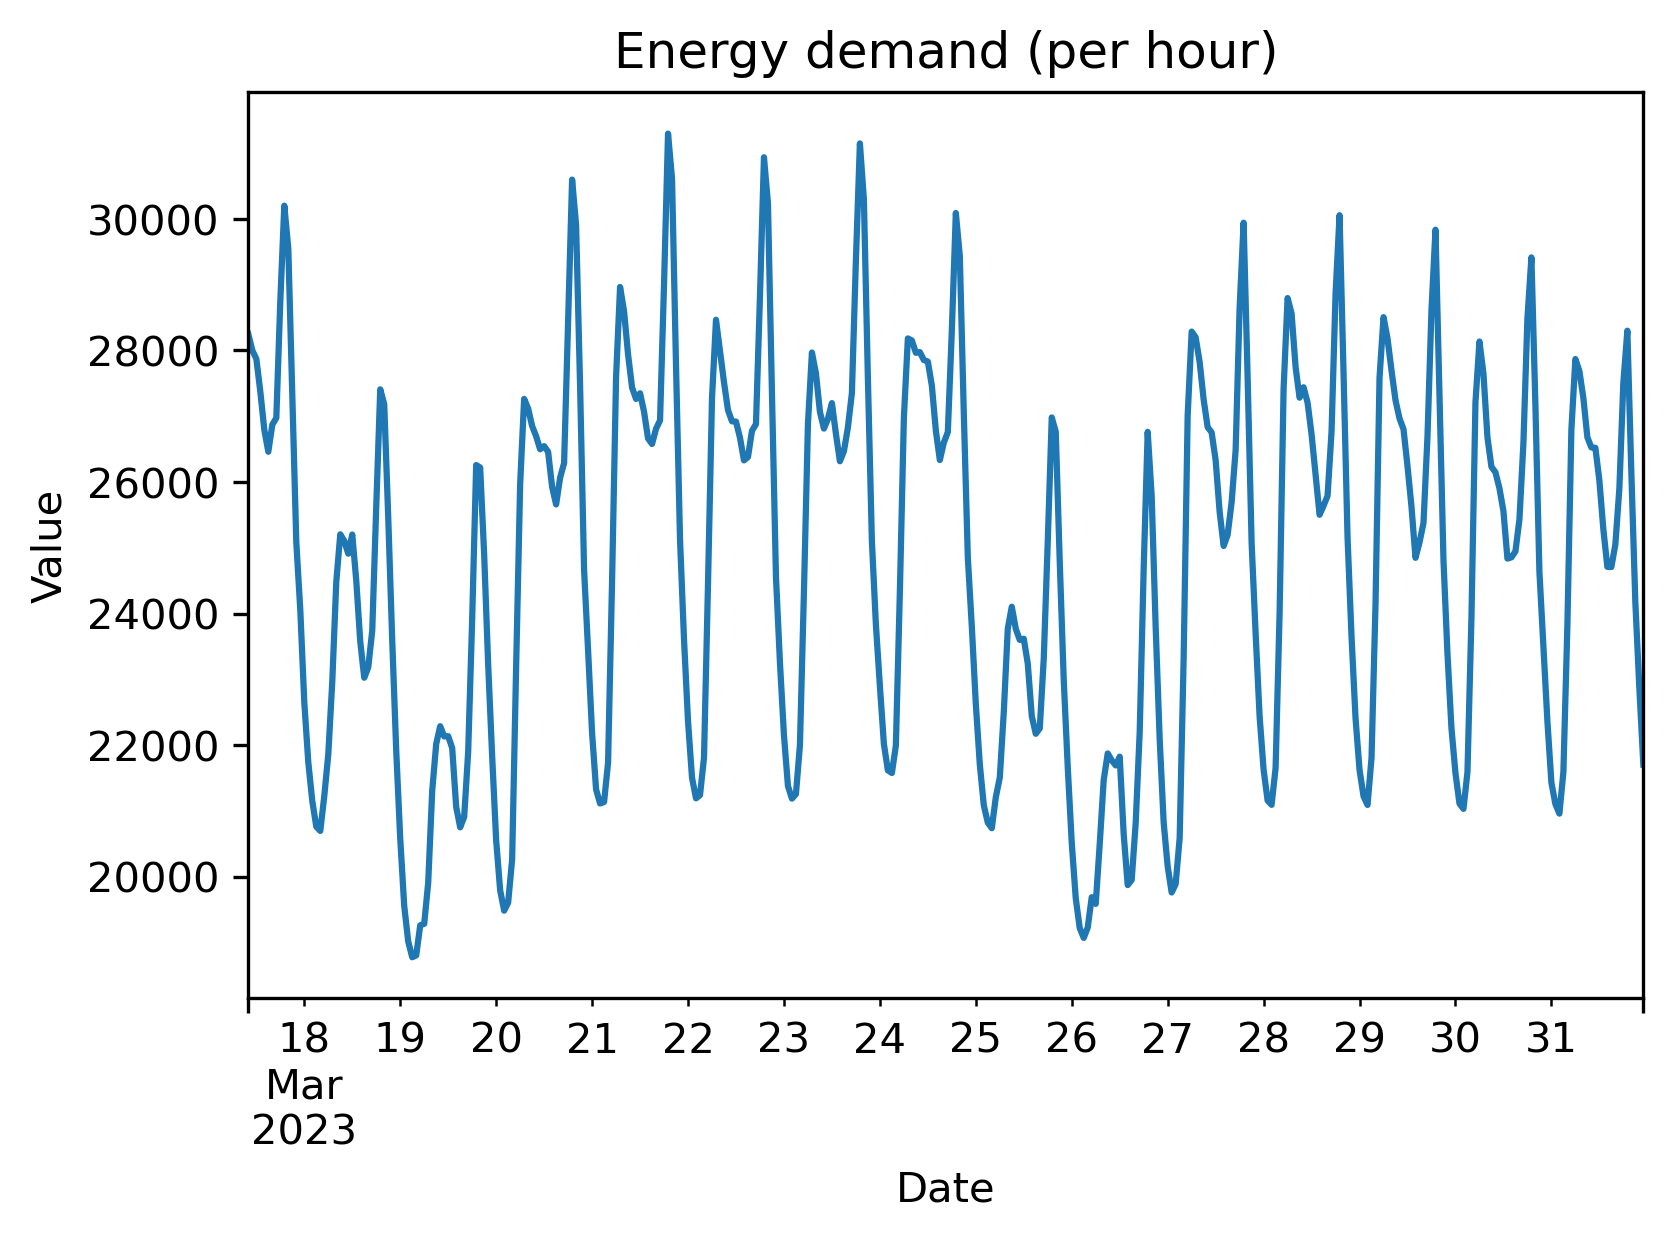
\includegraphics[width=1\linewidth]{images/variable_analysis/esios_demand_h_350}
        \caption{Per hour, 350 hours window.}
    \end{subfigure}
    \begin{subfigure}{.45\textwidth}
        \centering
        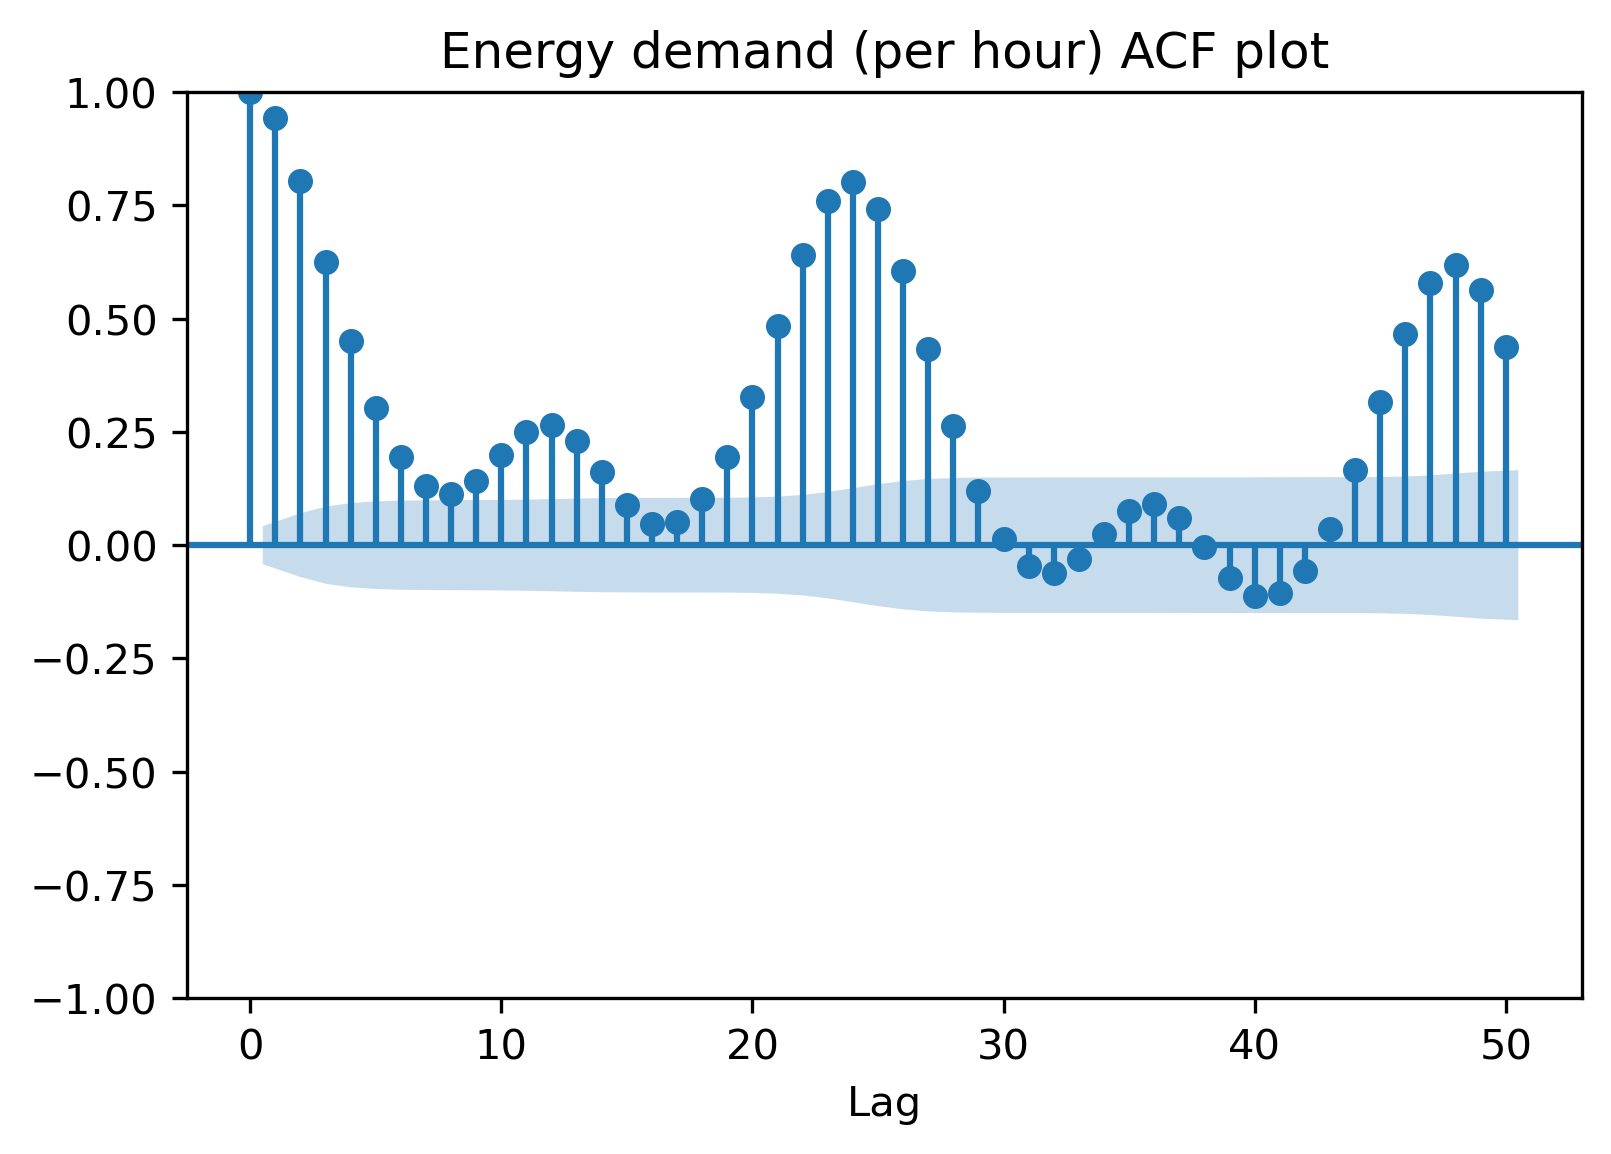
\includegraphics[width=1\linewidth]{images/variable_analysis/esios_demand_h_acf}
        \caption{Per hour, ACF plot.}
    \end{subfigure}
\end{figure}

\begin{figure}[H]\ContinuedFloat
    \begin{subfigure}{.44\textwidth}
        \centering
        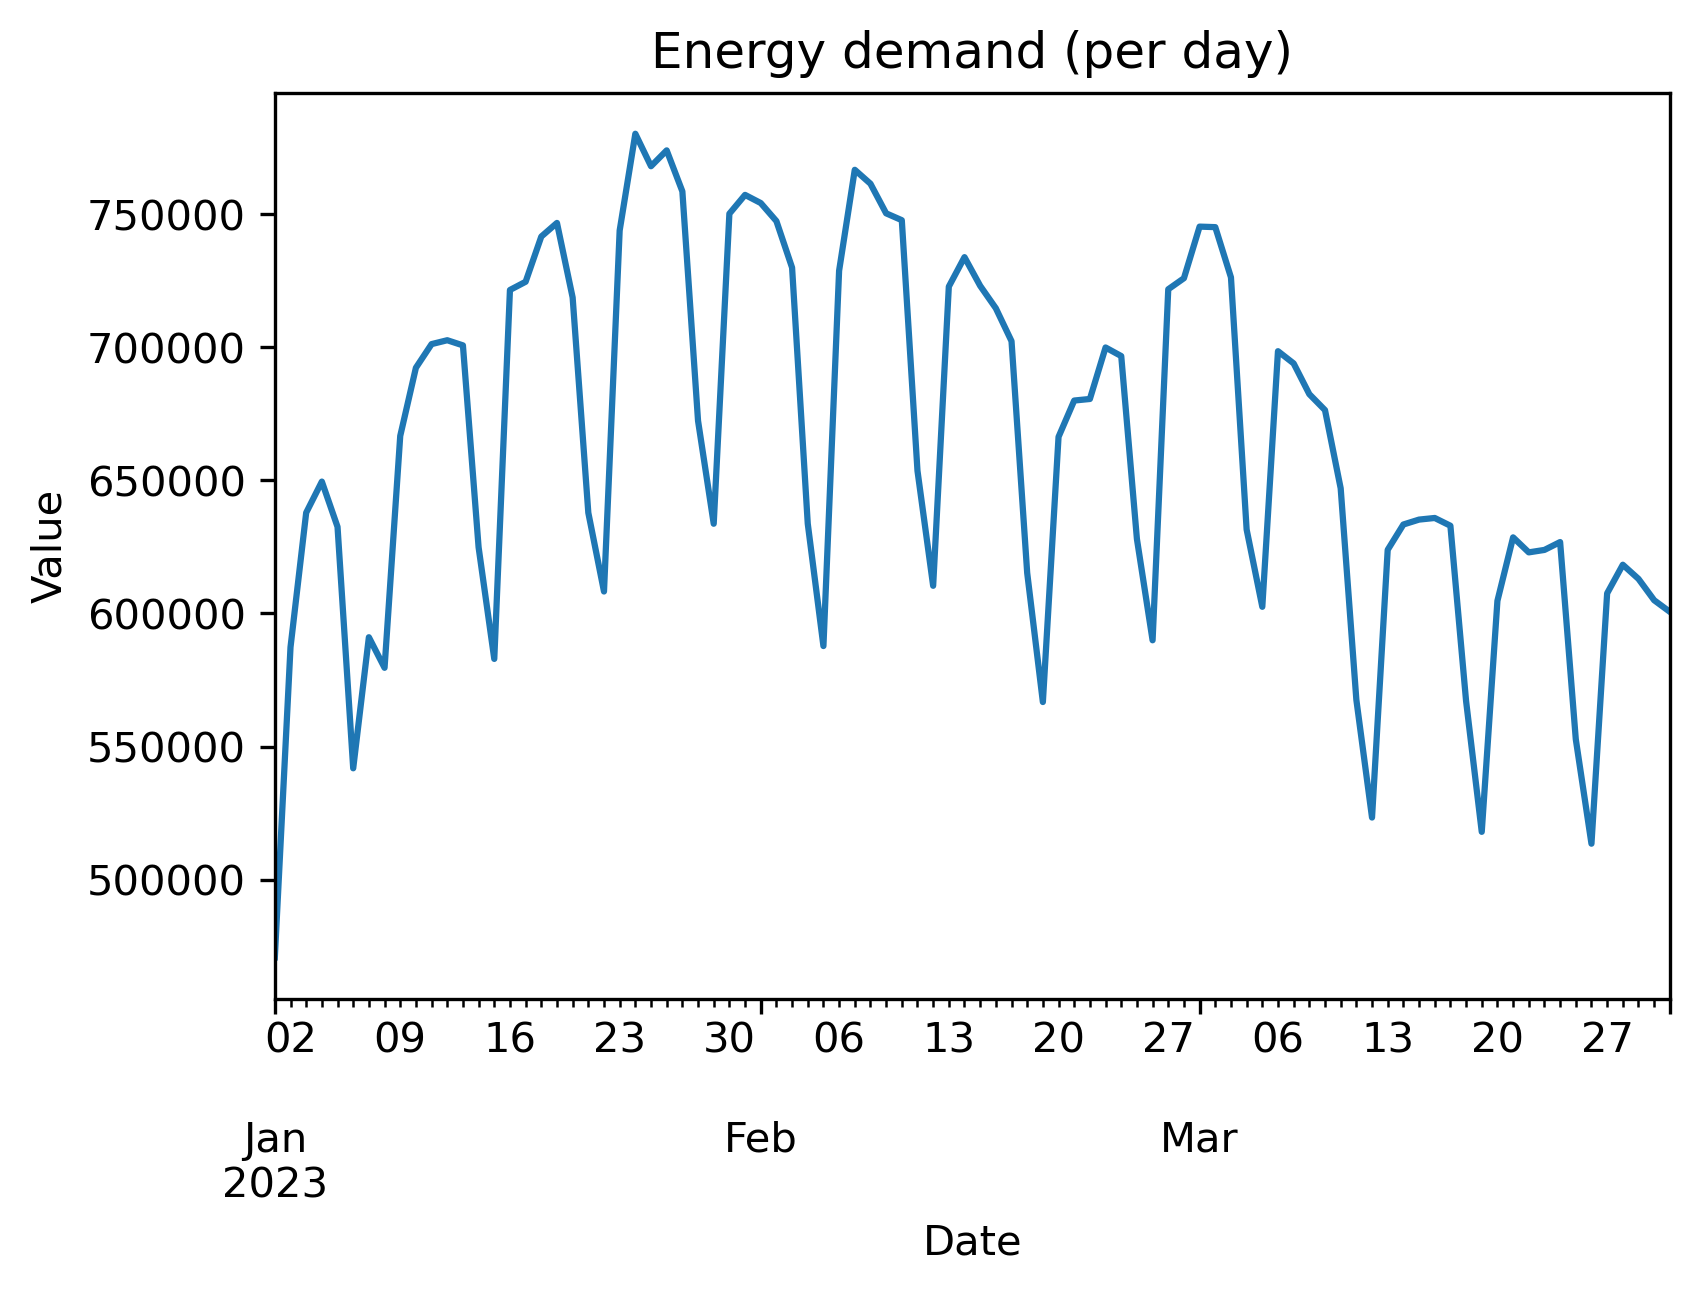
\includegraphics[width=1\linewidth]{images/variable_analysis/esios_demand_d_90}
        \caption{Aggregated by day, 90 days window.}
    \end{subfigure}
    \begin{subfigure}{.45\textwidth}
        \centering
        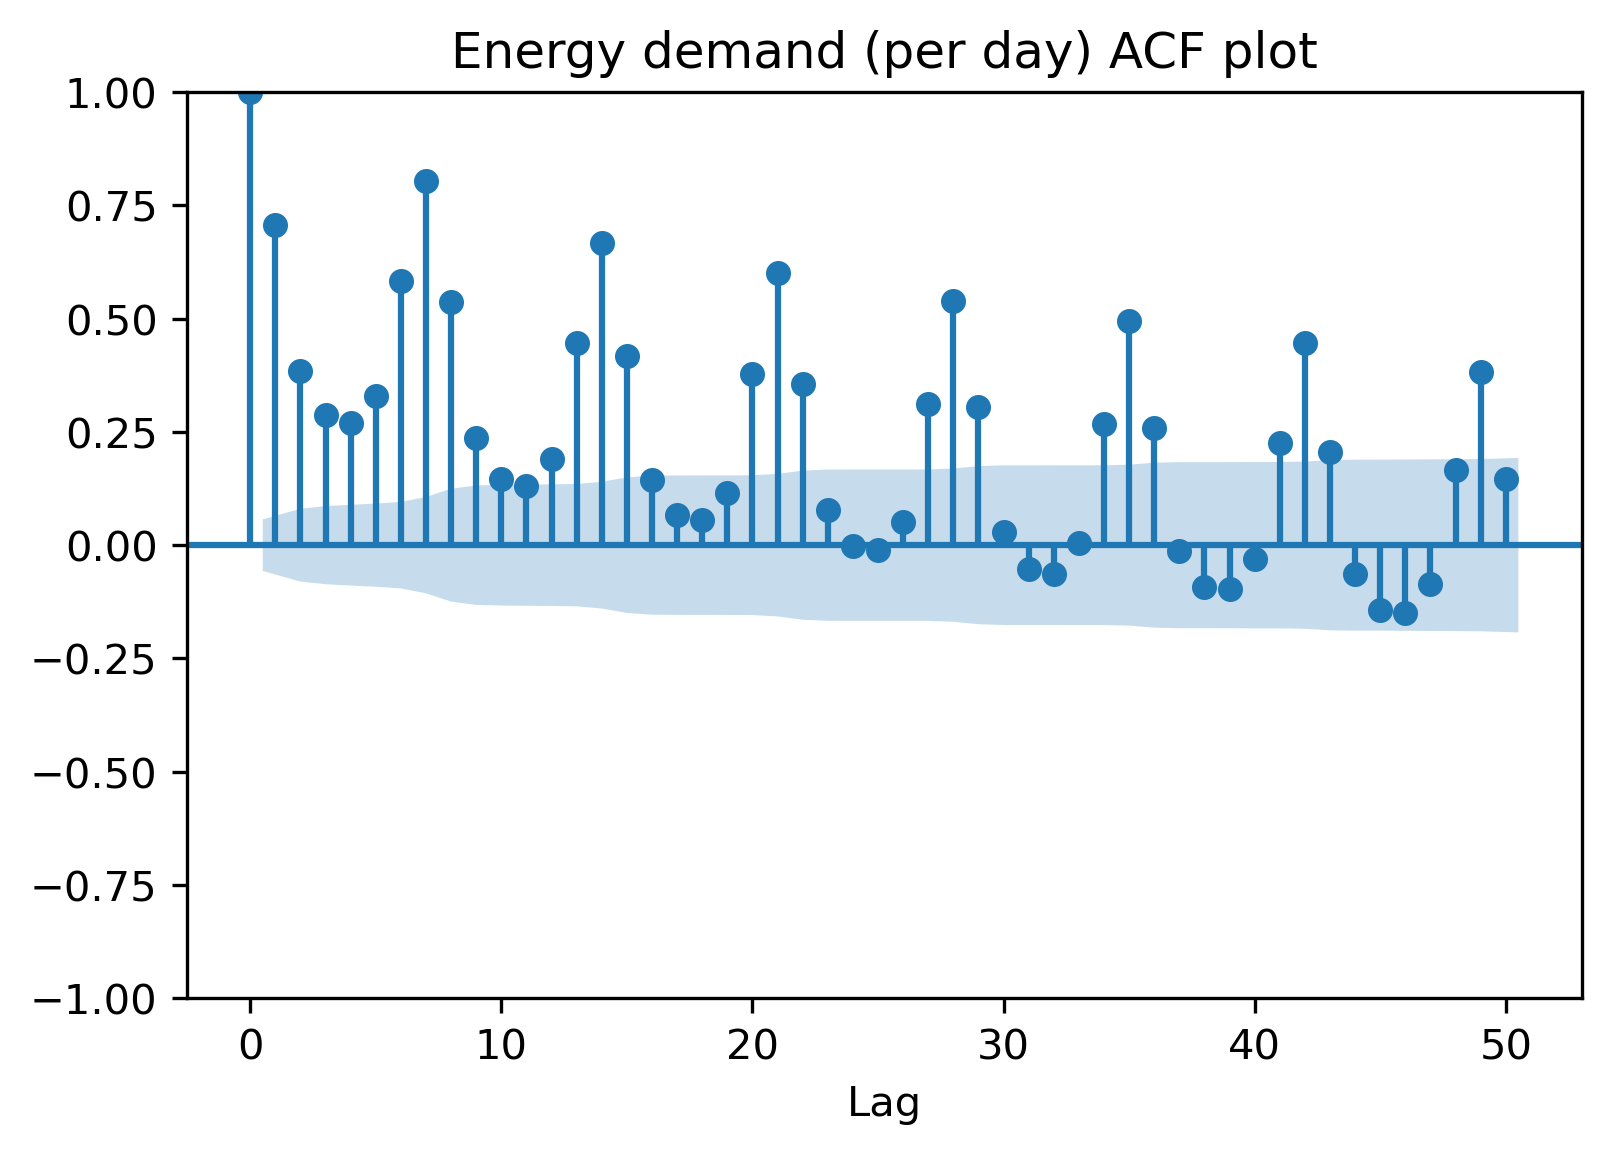
\includegraphics[width=1\linewidth]{images/variable_analysis/esios_demand_d_acf}
        \caption{Per day, ACF plot.}
    \end{subfigure}
\end{figure}

\begin{figure}[H]\ContinuedFloat
    \begin{subfigure}{.43\textwidth}
        \centering
        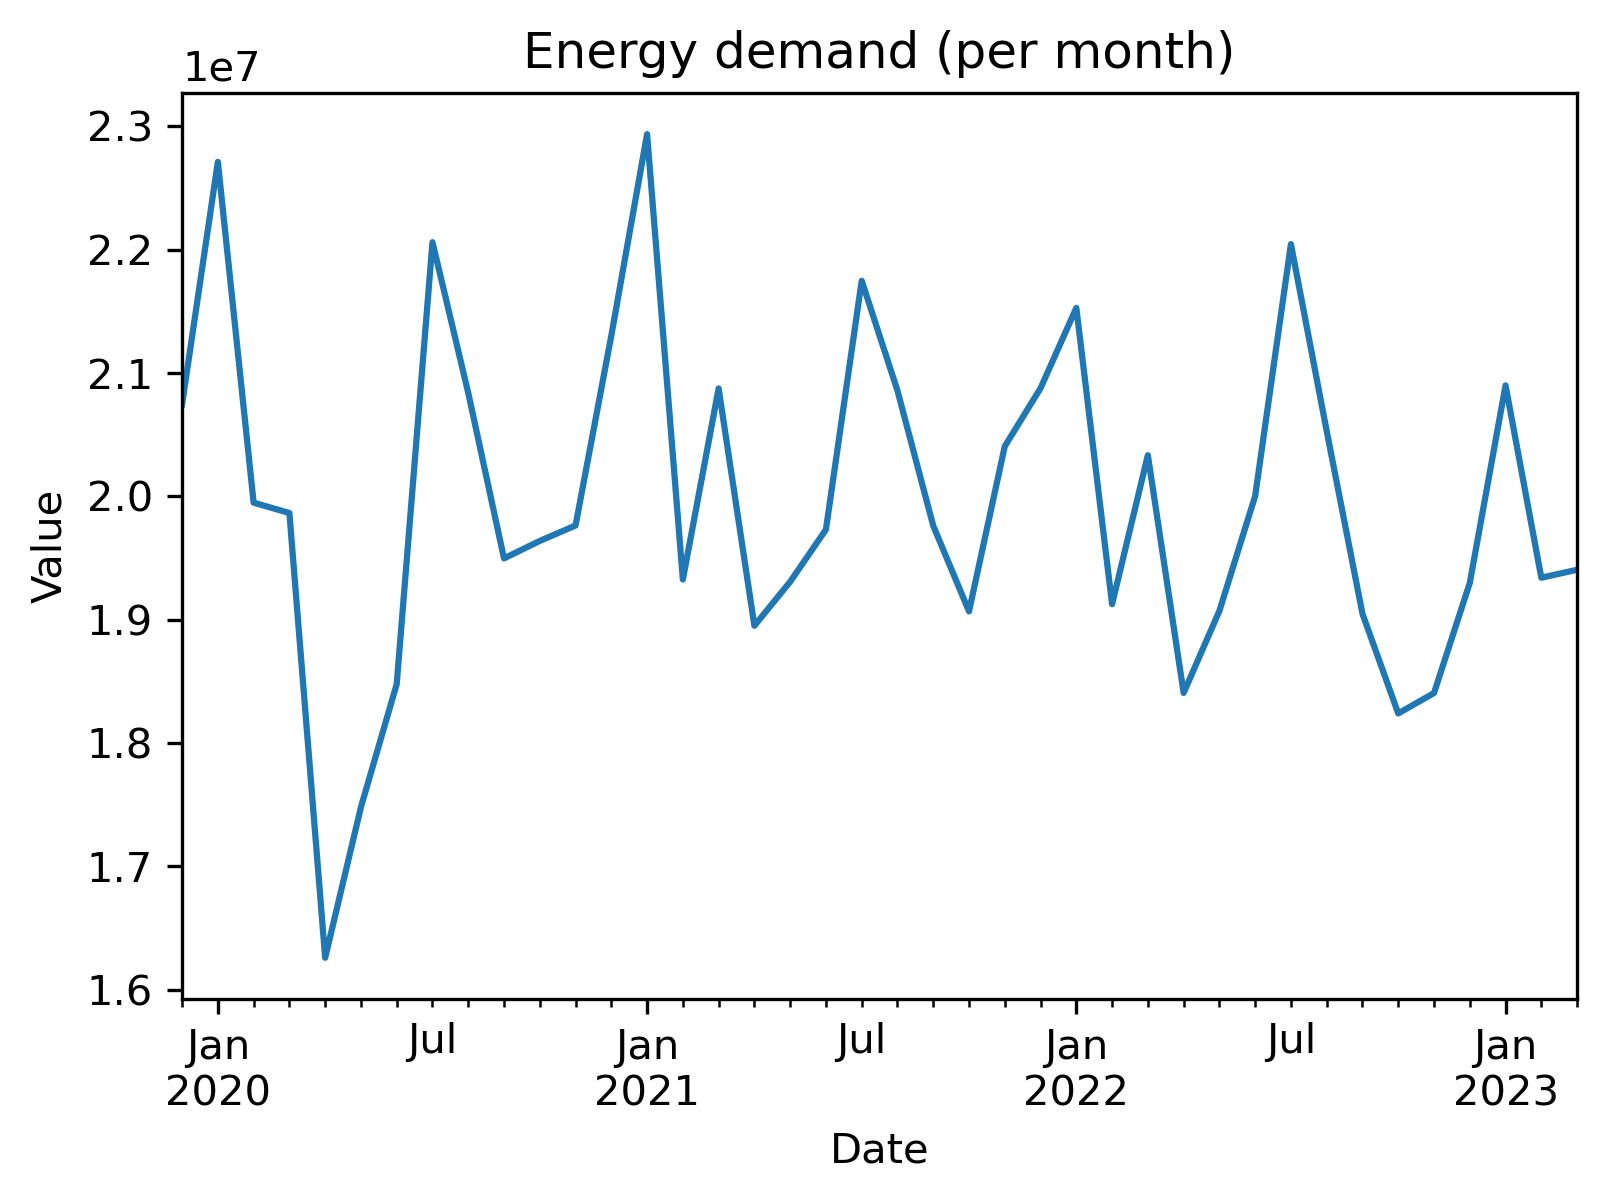
\includegraphics[width=1\linewidth]{images/variable_analysis/esios_demand_m_40}
        \caption{Aggregated by month, 40 months window.}
    \end{subfigure}
    \begin{subfigure}{.45\textwidth}
        \centering
        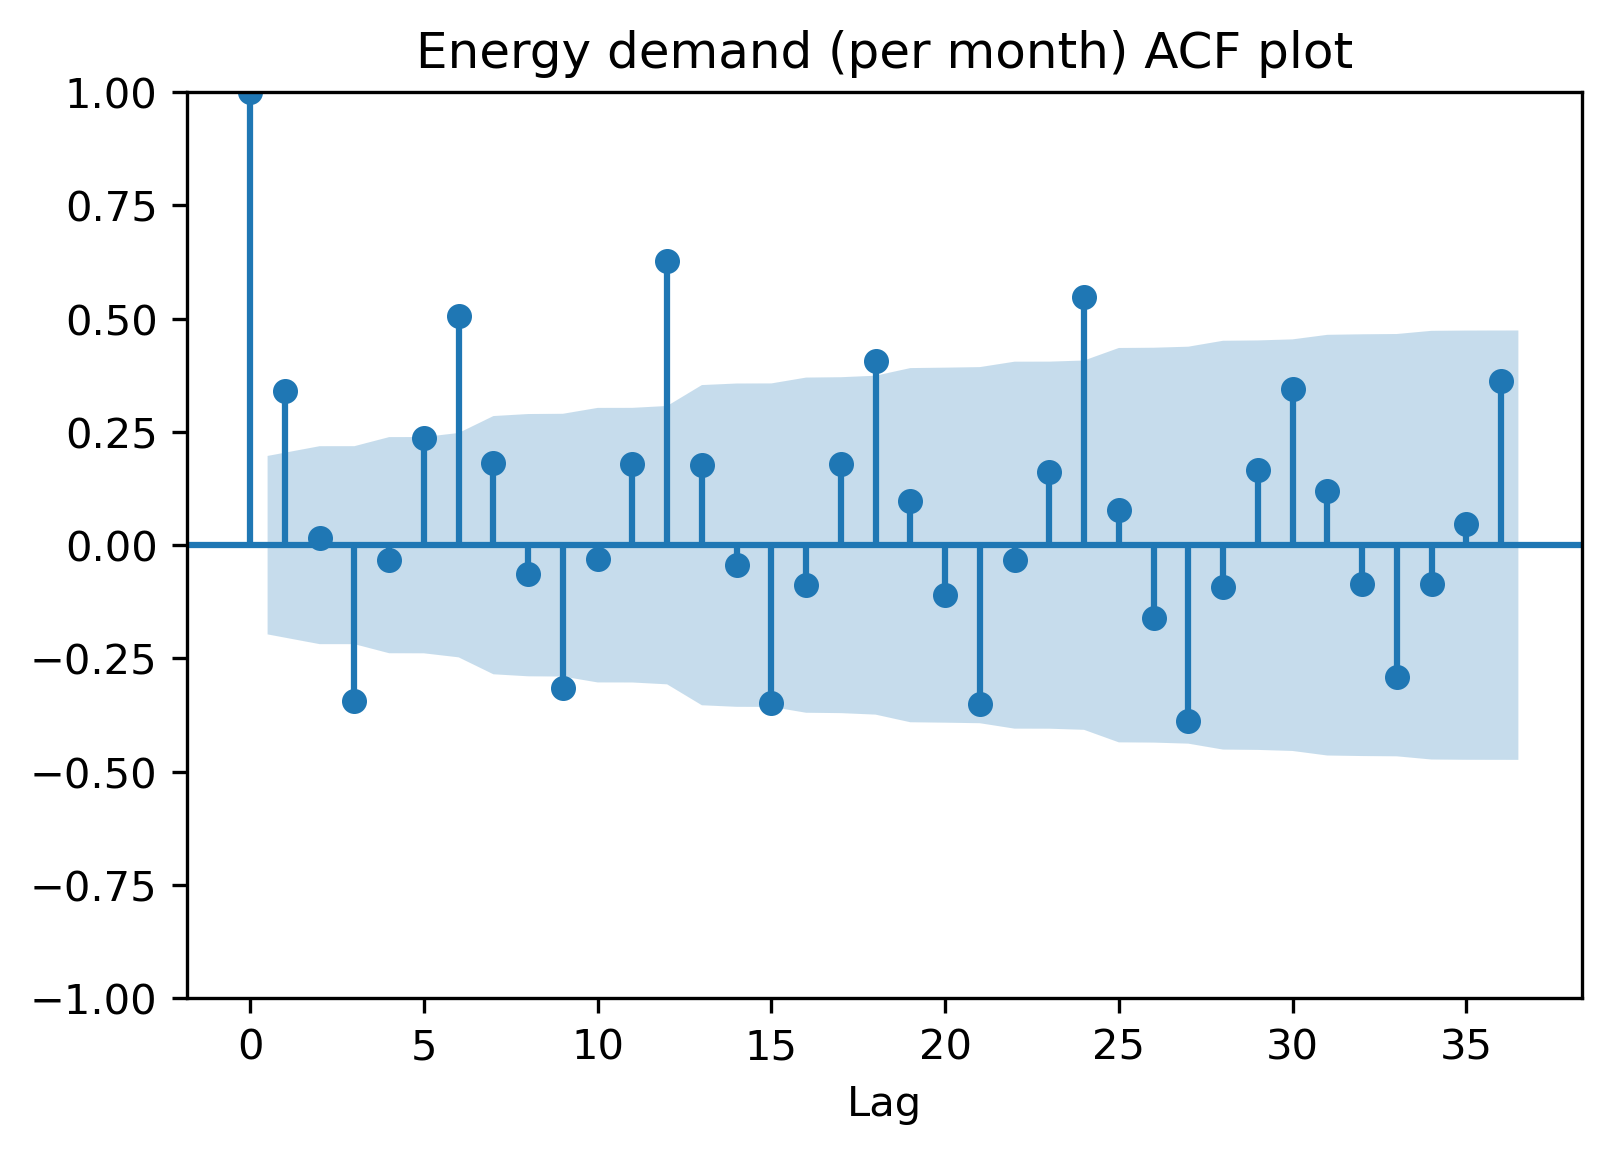
\includegraphics[width=1\linewidth]{images/variable_analysis/esios_demand_m_acf}
        \caption{Per month, ACF plot.}
    \end{subfigure}

    \caption{Electricity demand curves analysis.}
    \label{fig:demand-series}
\end{figure}

\subsection{Generation}
Energy generation involves the transformation of sources of primary energy into electricity.
The generation technologies differ in the way they produce the energy and in the primary energy they use for this task, each having different building and operation costs, technical characteristics and impact in the environment. \cite{subasta-electrica-totalenergies}

Demand and total generation are correlated, as the system operator is in charge of maintaining a balance between both.
There are generation technologies that always bid for a low price, even zero, as the nuclear: this is because a nuclear plant can't stop working, so it is always interested in selling the energy no matter the price.
Other as wind energy are also sold at a low price but not as low, because even though it is a cheap energy (the fuel is the own wind), the more you use a turbine the more maintenance it needs.
As it can be stopped, sometimes it is more adequate to do that than selling for zero.
Finally, technologies that tend to set the price of electricity are those using commodities, as combined cycles.

All the generation data has been downloaded from ESIOS in an hourly fashion.
We have downloaded generation data of the following technologies:
\begin{itemize}
    \item \textbf{Wind:} Existing yearly and half-yearly cyclicities have been found. This could make sense as wind may depend on temperature through the year. There is also a positive trend in the last years of wind energy generation.
    \item \textbf{Hydropower:} Strong daily cyclicity, with generation peaks in the hours with higher energy demand (Figures \ref{fig:hydro-series} and \ref{fig:hydro-acf}). There seems to be some weekly cyclicity but not very strong. The same happens in a yearly level.
    \item \textbf{Solar:} Really high daily cyclicity (Figure \ref{fig:solar-acf}). Cyclicity also in a yearly fashion, with a positive trend in the solar energy generation in the previous years (Figure \ref{fig:solar-series}).
    \item \textbf{Nuclear:} In the short term it is a very stable energy technology, with not many generation changes between nearby hours, see Figure \ref{fig:nuclear-series}. Maybe some cycles appear in a yearly and half-yearly fashion, but they are not very clear. There is no trend in the long term for the generation with this technology.
    \item \textbf{Combined cycles:} This technology, powered by gas, uses the combustion to move turbines. Apart, the residual heat is used to heat water and move other turbines, increasing generation efficiency. There exists some cyclicity in half-daily, daily and weekly horizons.
    \item \textbf{Coal:} This raw material has been a very popular fuel in thermal power plants, but in the previous years its use has decreased a lot due to how pollutant is. As can be seen in Figure \ref{fig:coal-series}, the use of coal as generation fuel has decreased a lot in the last years.
\end{itemize}

\begin{figure}[H]
\centering
    \begin{subfigure}{.43\textwidth}
        \centering
        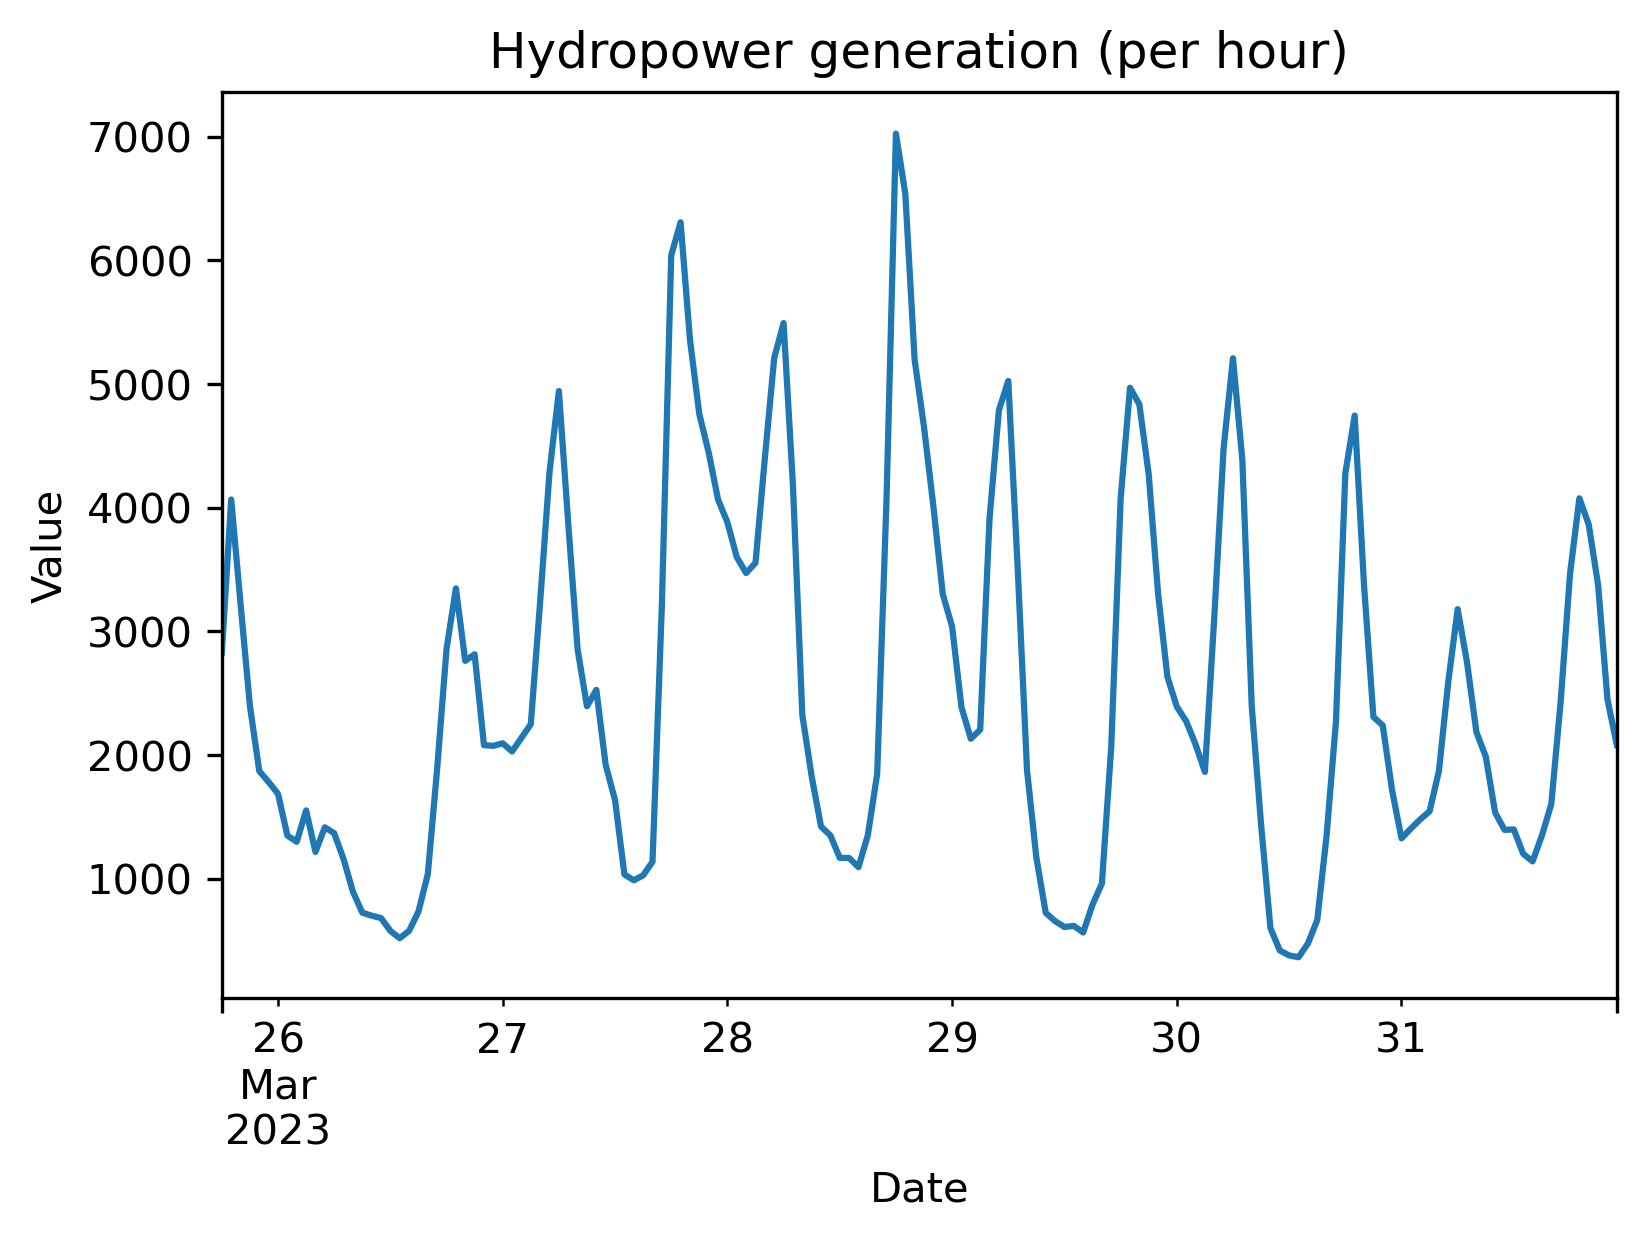
\includegraphics[width=1\linewidth]{images/variable_analysis/esios_generation_hydro_h_96}
        \caption{Hydropower per hour, 350 hours window.}
        \label{fig:hydro-series}
    \end{subfigure}
    \begin{subfigure}{.45\textwidth}
        \centering
        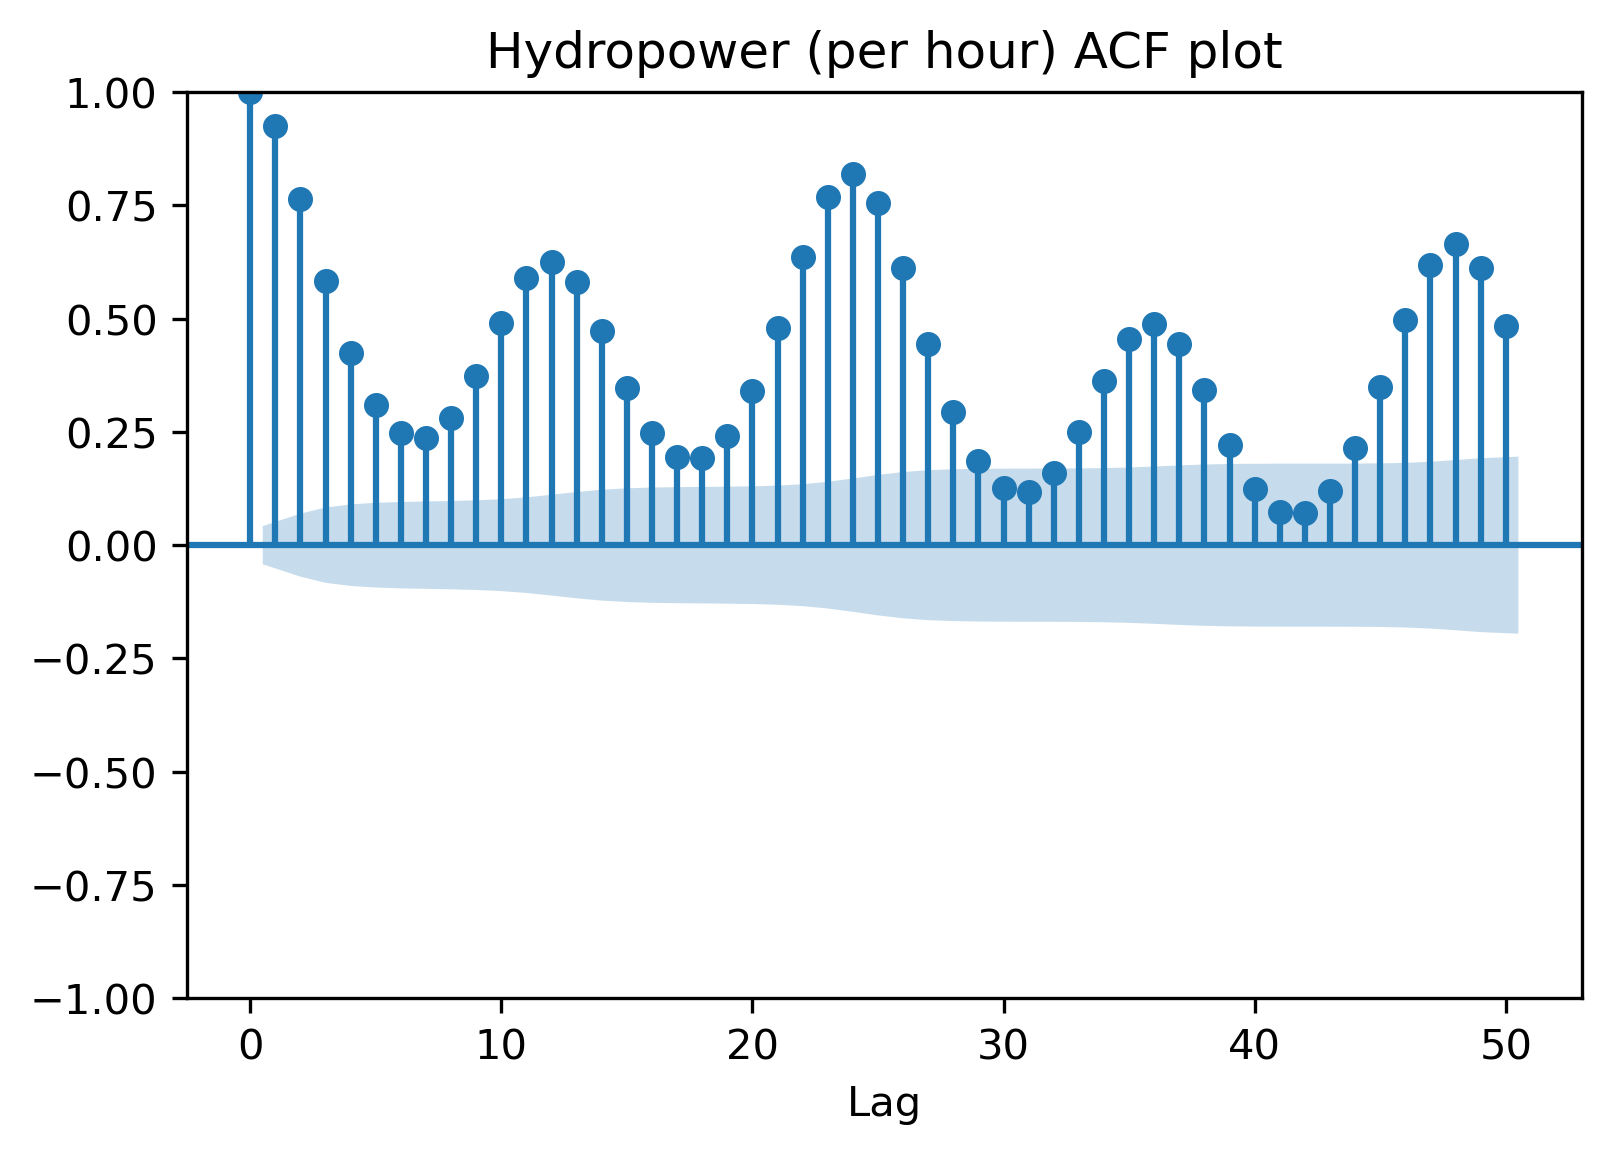
\includegraphics[width=1\linewidth]{images/variable_analysis/esios_generation_hydro_h_acf}
        \caption{Hydropower per hour, ACF plot.}
        \label{fig:hydro-acf}
    \end{subfigure}
\end{figure}

\begin{figure}[H]\ContinuedFloat
    \begin{subfigure}{.44\textwidth}
        \centering
        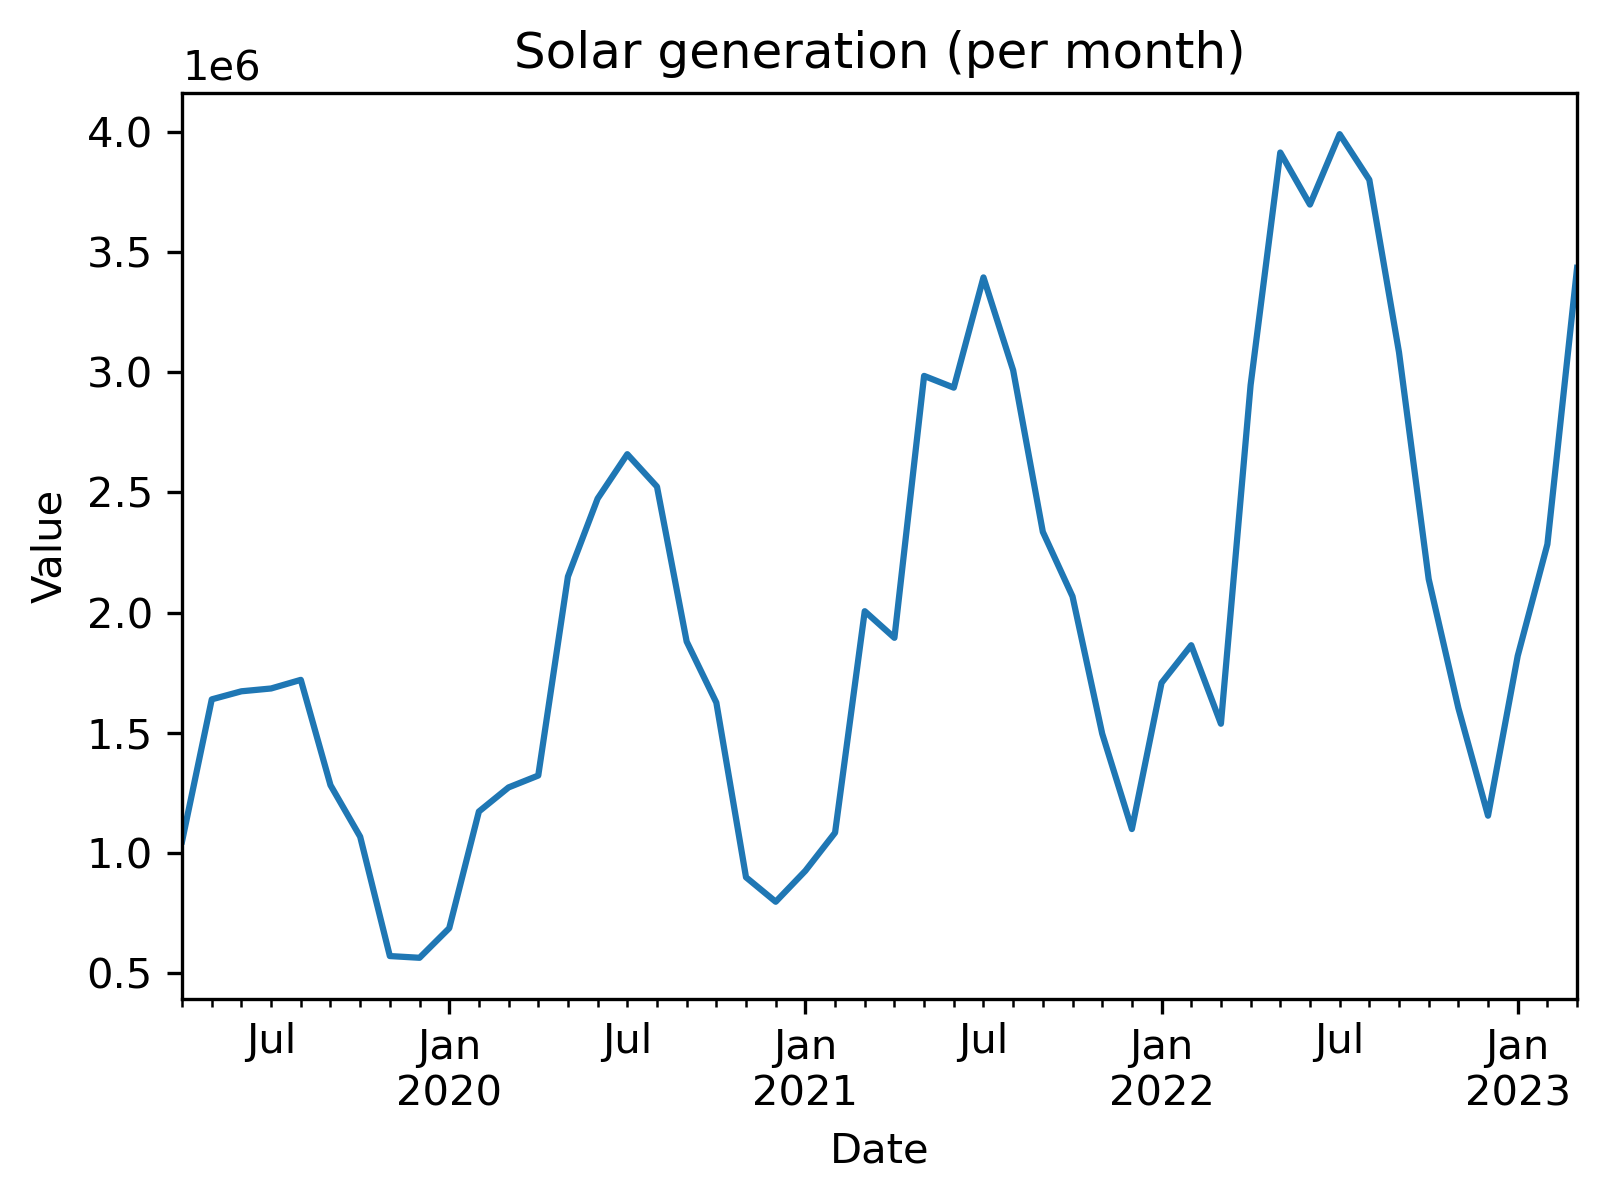
\includegraphics[width=1\linewidth]{images/variable_analysis/esios_generation_solar_m_48}
        \caption{Solar aggregated by day, 90 days window.}
        \label{fig:solar-series}
    \end{subfigure}
    \begin{subfigure}{.45\textwidth}
        \centering
        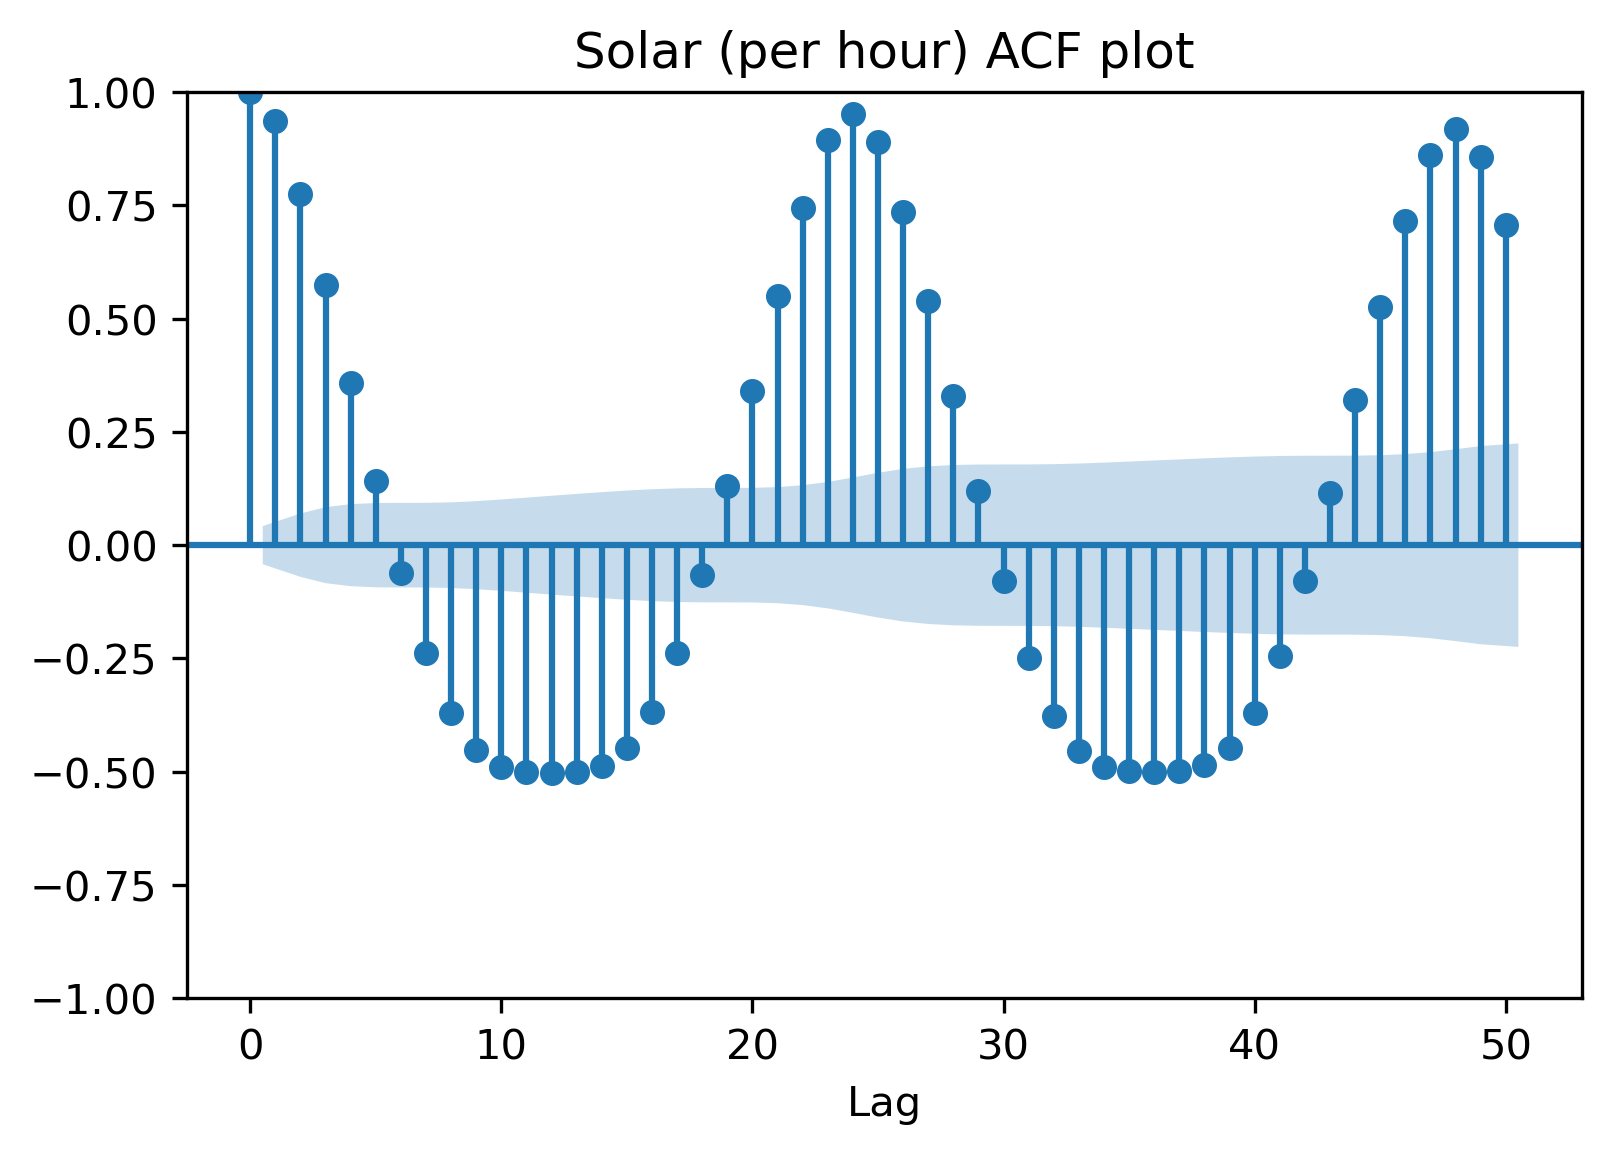
\includegraphics[width=1\linewidth]{images/variable_analysis/esios_generation_solar_h_acf}
        \caption{Solar per day, ACF plot.}
        \label{fig:solar-acf}
    \end{subfigure}
\end{figure}

\begin{figure}[H]\ContinuedFloat
    \begin{subfigure}{.43\textwidth}
        \centering
        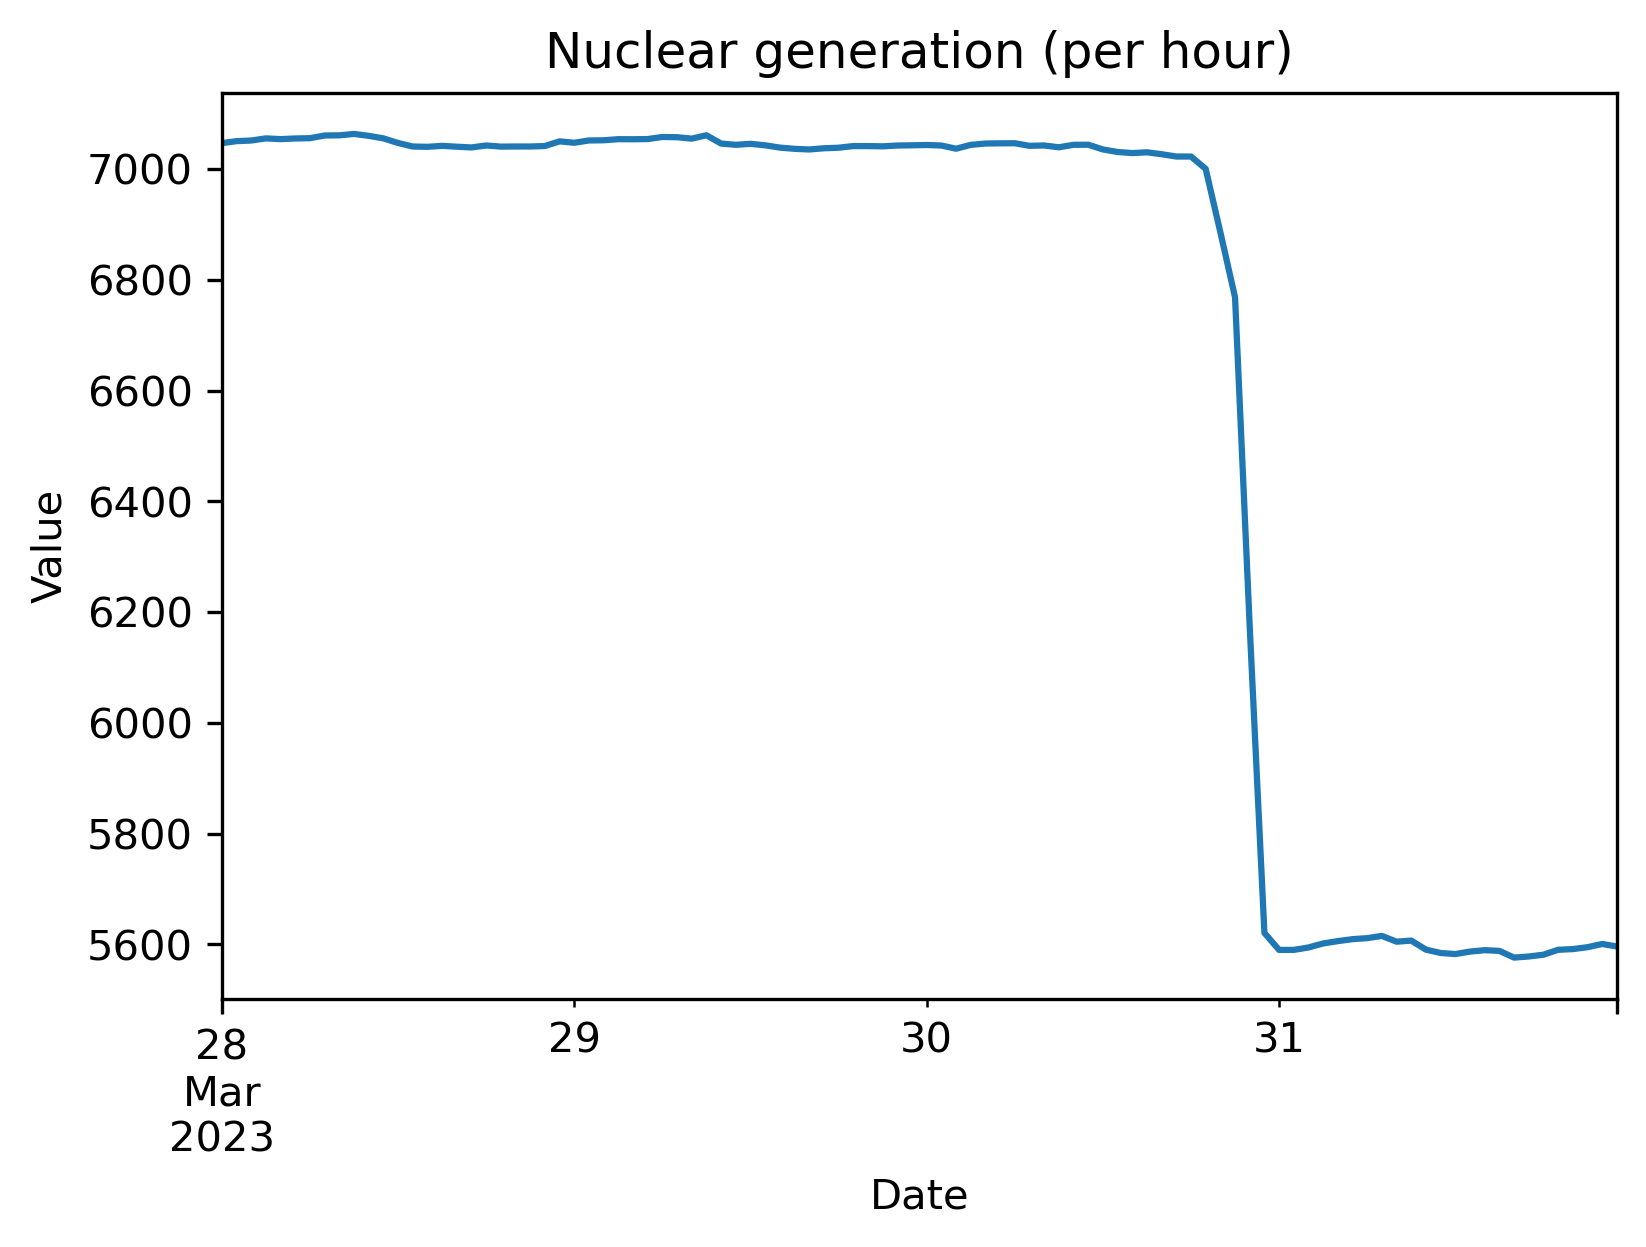
\includegraphics[width=1\linewidth]{images/variable_analysis/esios_generation_nuclear_h_96}
        \caption{Nuclear agg. by month, 40 months window.}
        \label{fig:nuclear-series}
    \end{subfigure}
    \begin{subfigure}{.47\textwidth}
        \centering
        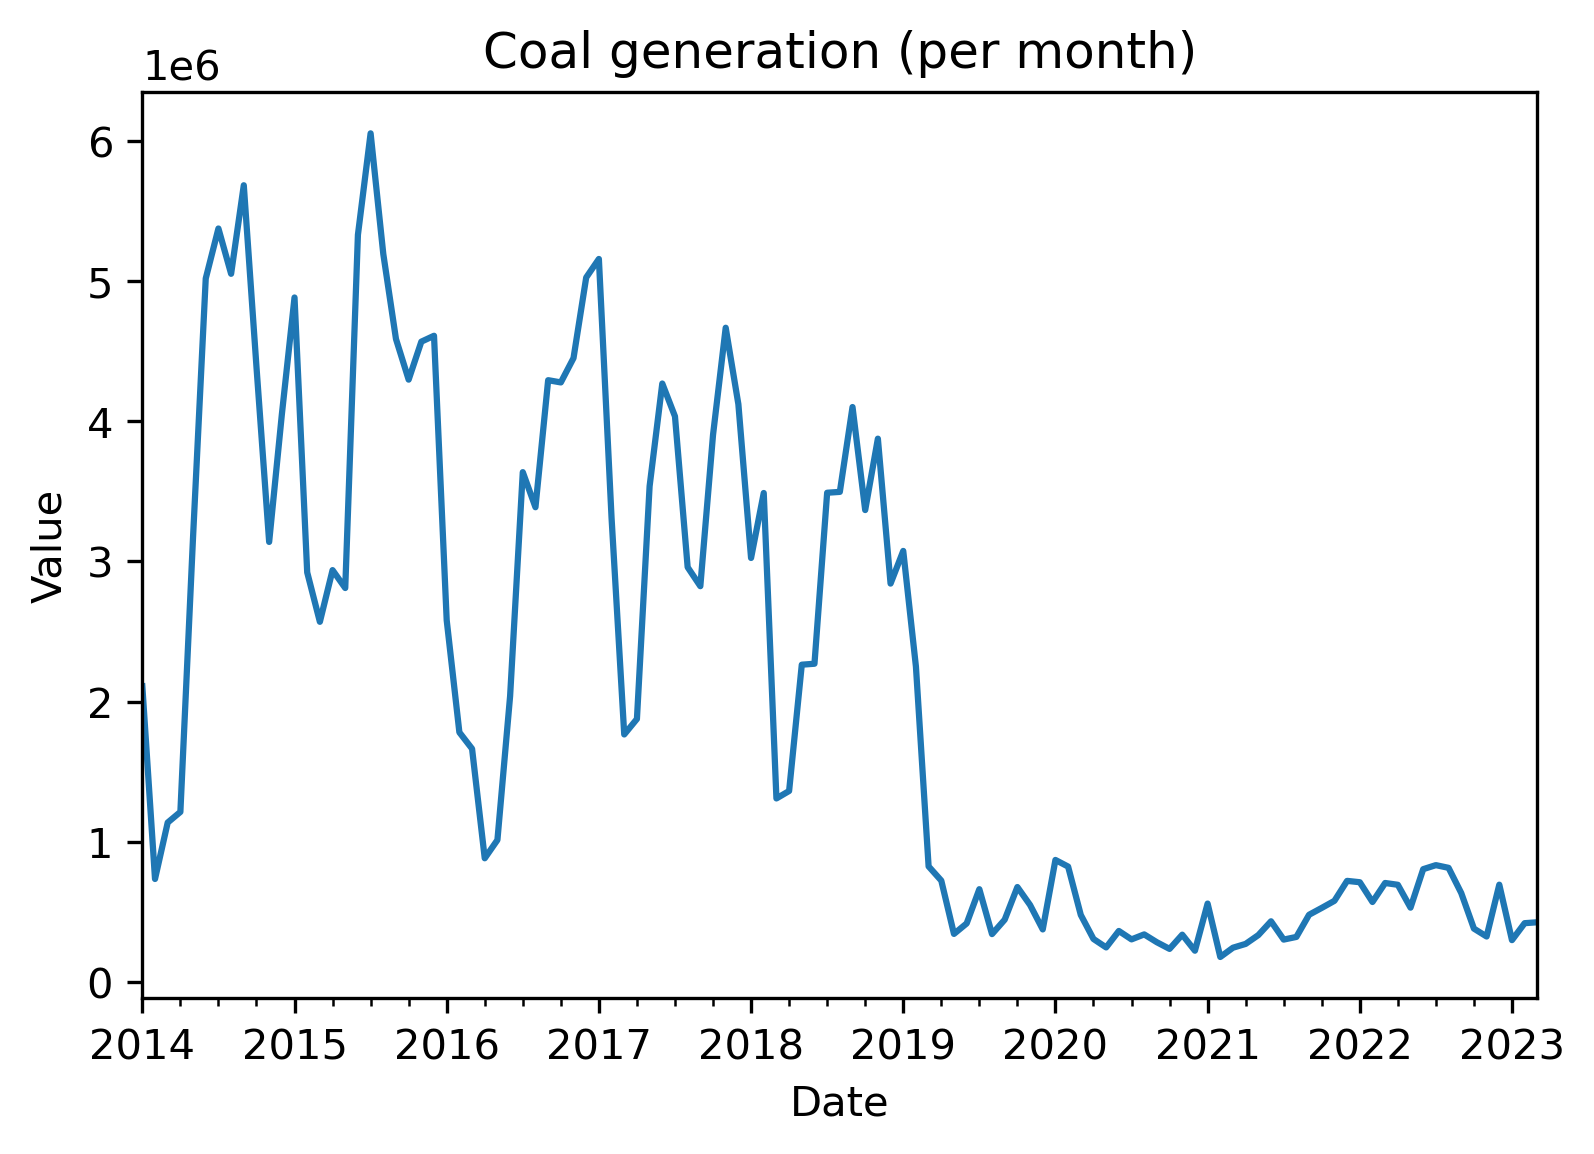
\includegraphics[width=1\linewidth]{images/variable_analysis/esios_generation_coal_m_all}
        \caption{Coal per month, complete series.}
        \label{fig:coal-series}
    \end{subfigure}

    \caption{Electricity demand curves analysis.}
    \label{fig:generation-series}
\end{figure}


\subsection{Price of commodities}
As the technologies using commodities to make energy usually set the market price, the price of these commodities could be also affecting it.
The author will study the influence of coal and gas.

Concretely, the gas prices in use will be the ones dictated by the TTF index, which have been downloaded from investing.com: from 10-2017 to 04-2023 in a daily fashion and from 04-2010 to 03-2023 in a yearly granularity. In the monthly case, the author works with the last observation in the month: that is because this is the only measure provided in the source, apart from minimum and maximum values in the period.

For the coal prices we will use the ARGUS/McCloskey index. Data has been downloaded from marketwatch.com, daily readings from 12-2010 to 03-2023.

As happened with electricity price, in Figure \ref{fig:commodities-series} we find a peak in prices in 2021 and 2022.

\begin{figure}[H]
\centering
    \begin{subfigure}{.45\textwidth}
        \centering
        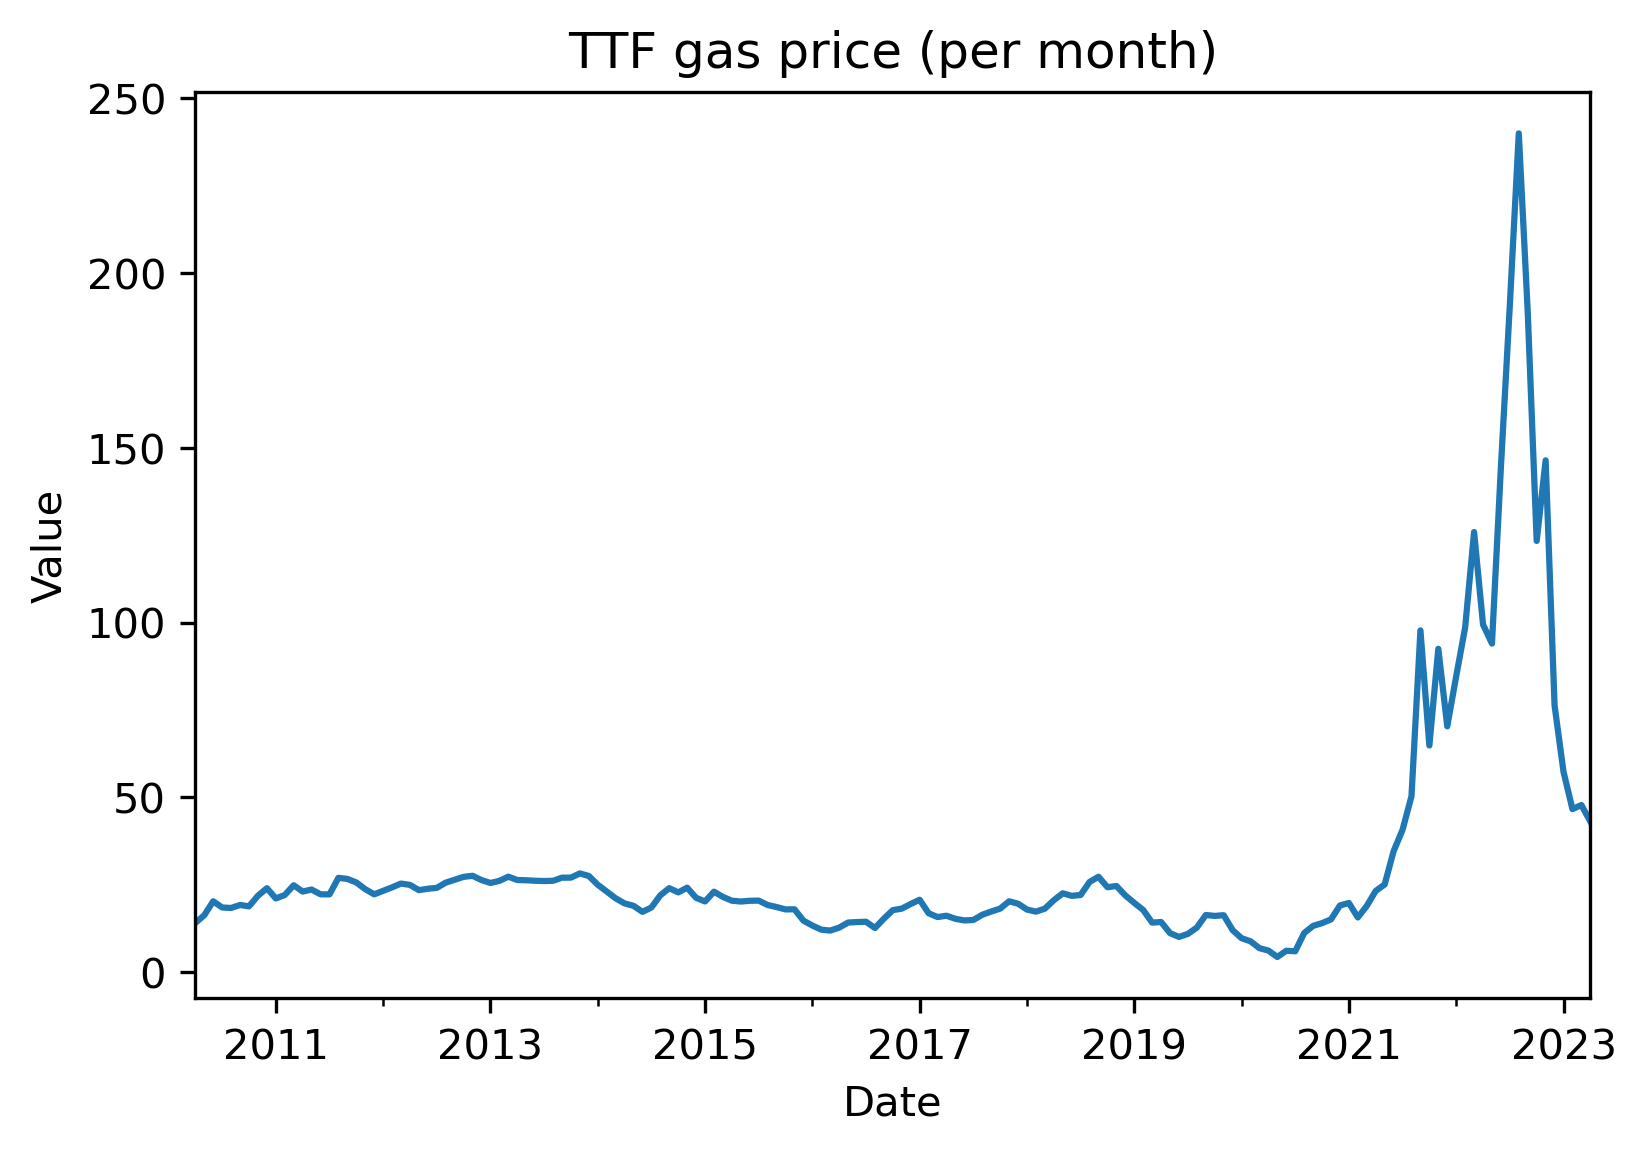
\includegraphics[width=1\linewidth]{images/variable_analysis/ttf_m_all}
        \caption{TTF gas price curve.}
    \end{subfigure}
    \begin{subfigure}{.45\textwidth}
        \centering
        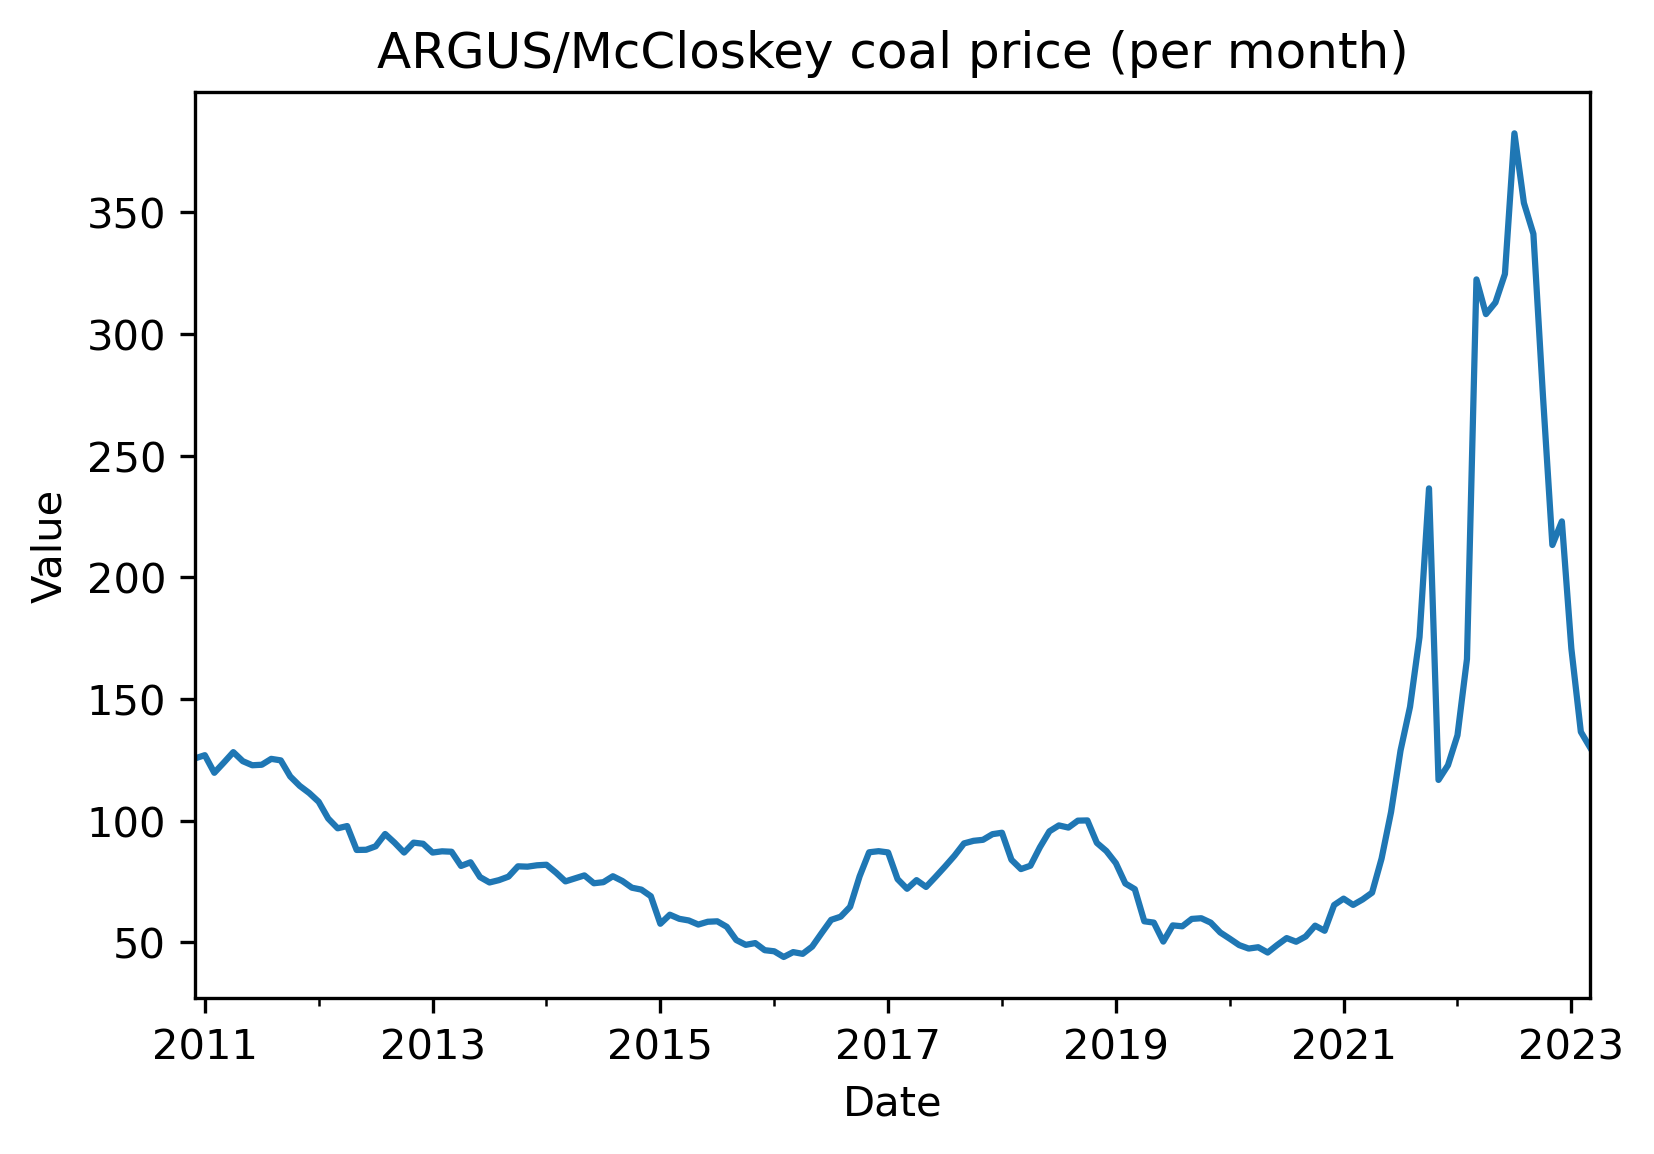
\includegraphics[width=1\linewidth]{images/variable_analysis/coal_m_all}
        \caption{ARGUS/McCloskey coal price curve.}
    \end{subfigure}

    \caption{Gas and coal price curves.}
    \label{fig:commodities-series}
\end{figure}

\subsection{EU Allowances (EUAs)}
The use of technologies producing carbon emissions requires to pay taxes to the European Union.
Companies buy allowances to be able to emmit $CO_2$ and they can trade with them, that's why allowances have market value which can influence the cost of energy.

The price of this allowance has been downloaded from International Carbon Action Partnership, having daily entries from 12-2010 to 03-2023. Monthly aggregated values are plotted in Figure \ref{fig:c02-euas-series}, we find an increase in its price in the previous years.

\subsection{Macroeconomic variables}
The economic situation affects prices in general, and therefore it can affect electricity cost.
GDP or inflation could be potential indicators to study. The author has chosen to study Spanish GDP downloading data from the World Bank, concretely from 1960 to 2021. We see an increasing trend for it in Figure \ref{fig:gdp-series}.

\begin{figure}[H]
\centering
    \begin{subfigure}{.45\textwidth}
        \centering
        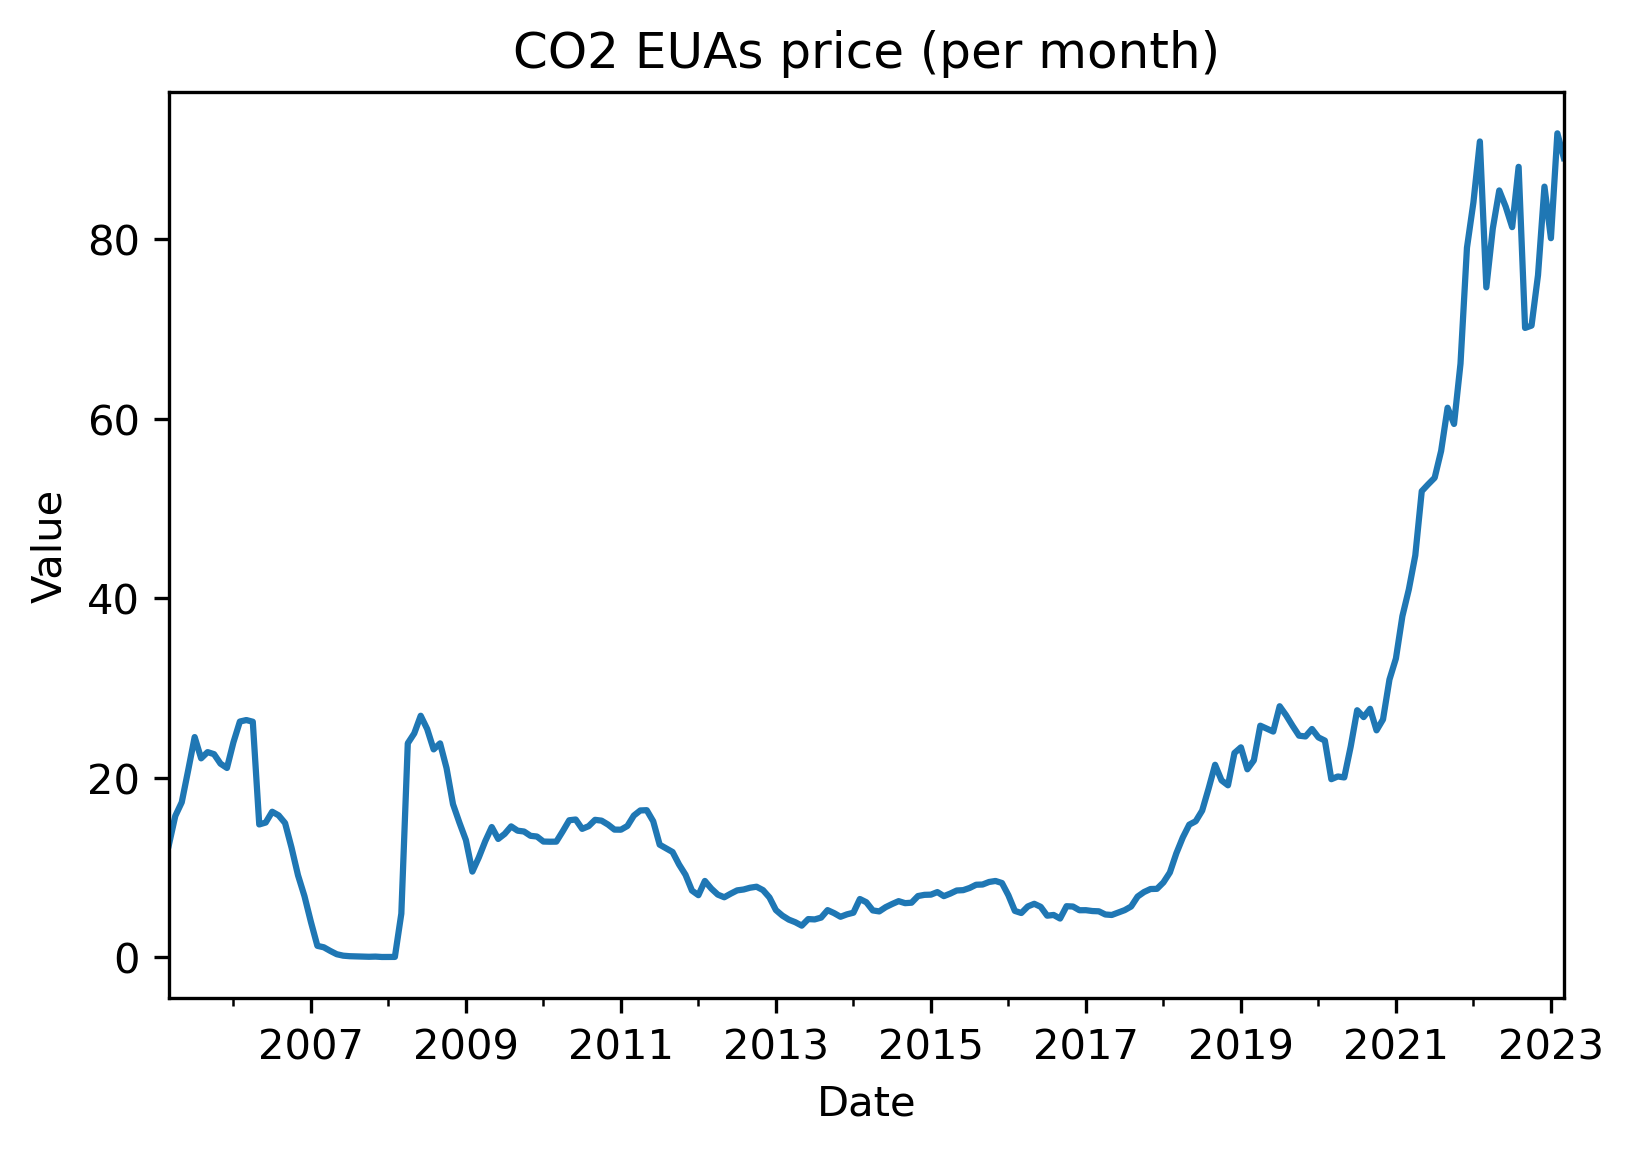
\includegraphics[width=1\linewidth]{images/variable_analysis/co2_m_all}
        \caption{CO2 European Allowances price.}
        \label{fig:c02-euas-series}
    \end{subfigure}
    \begin{subfigure}{.45\textwidth}
        \centering
        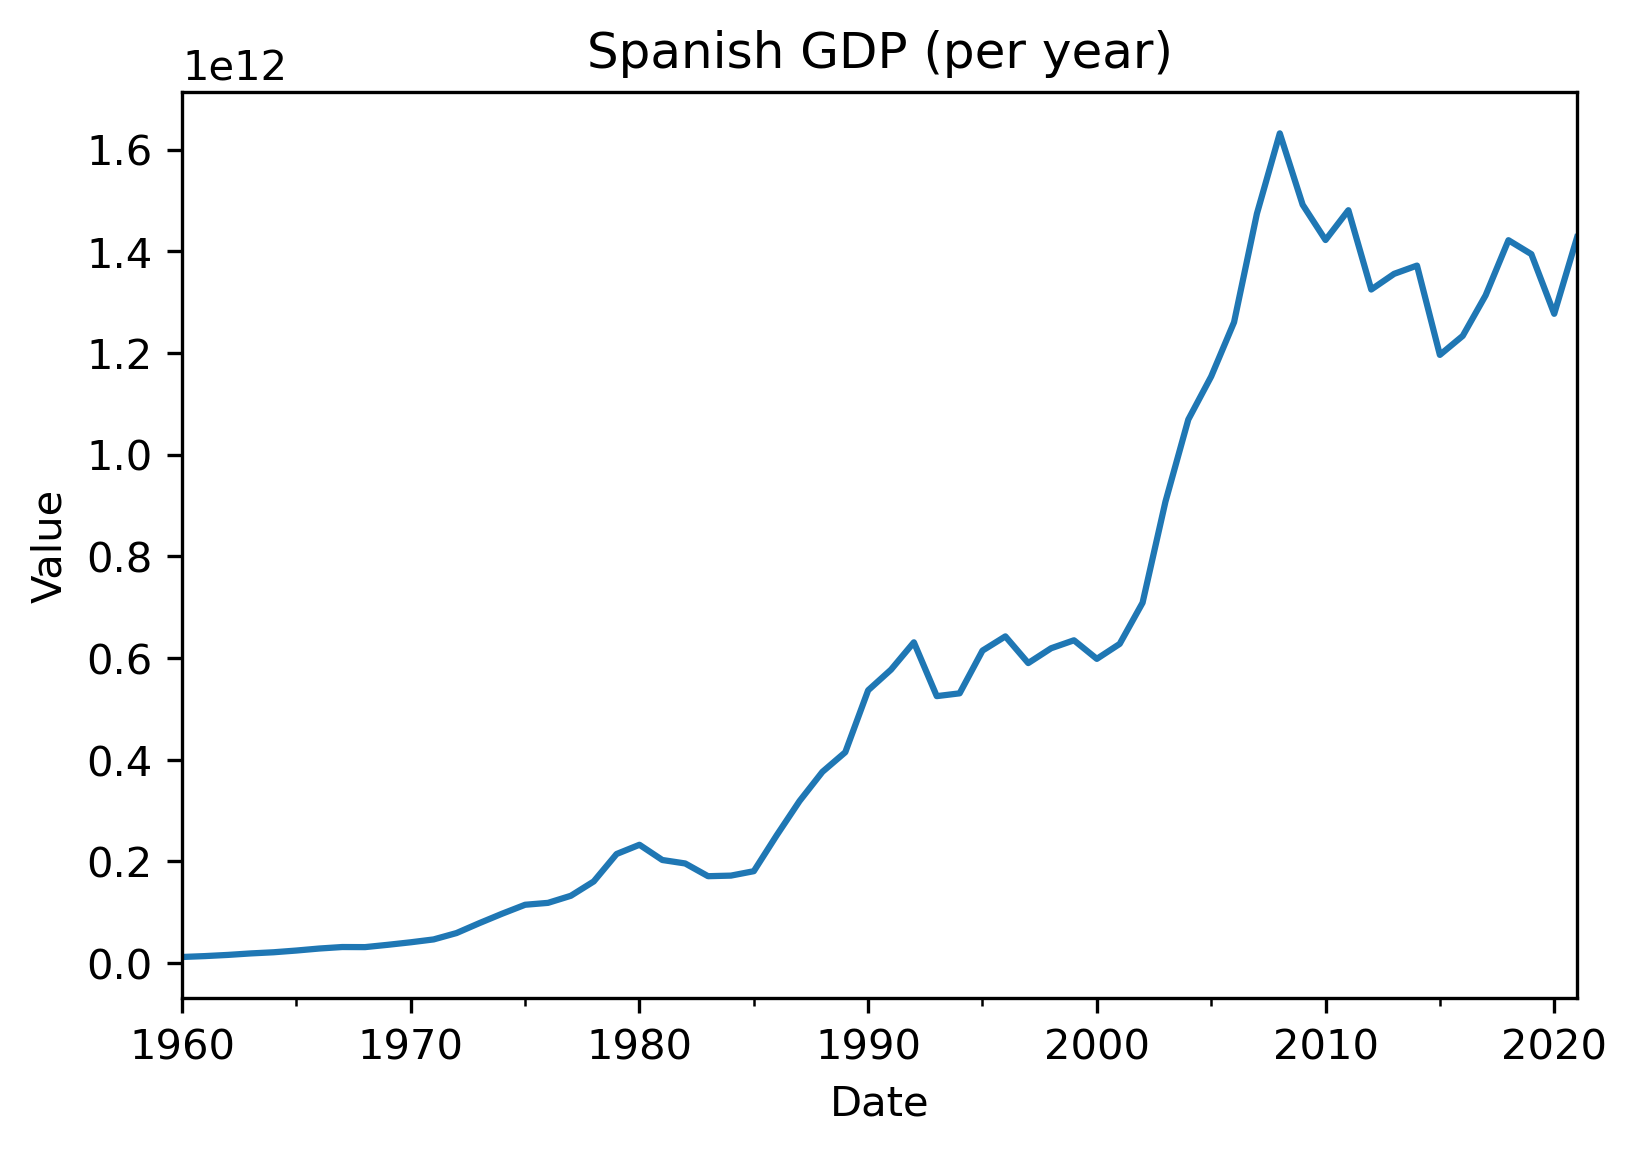
\includegraphics[width=1\linewidth]{images/variable_analysis/gdp_y_all}
        \caption{Spanish GDP.}
        \label{fig:gdp-series}
    \end{subfigure}

    \caption{CO2 EUAs and Spanish GDP series.}
    \label{fig:co2-gdp-analysis}
\end{figure}

\subsection{Time of day/week}
Something to consider is the moment for which the predictions are done.
The price is not the same during the day or night, or in weekdays or weekends.
This is correlated with the demand and the availability of renewable energy generation.

\vspace{1.3cm}

The previous predictors can improve the model capabilities, as they could add extra explicative information about the price.
In the next sections the author will analyze which of them are explaining the most in the specific studied models.

